\documentclass[sensors,article,submit,pdftex,moreauthors]{Definitions/mdpi}
%DIF LATEXDIFF DIFFERENCE FILE
%DIF DEL old.tex   Thu May 28 14:28:56 2026
%DIF ADD new.tex   Thu May 28 18:44:59 2026
\firstpage{1}
\makeatletter
\setcounter{page}{\@firstpage}
\makeatother
\pubvolume{1}
\issuenum{1}
\articlenumber{0}
\pubyear{2026}
\copyrightyear{2026}
\externaleditor{Academic Editor: Firstname Lastname}
\datereceived{}
\daterevised{}
\dateaccepted{}
\datepublished{}
%\hreflink{https://www.mdpi.com/journal/sensors}

\usepackage{amsmath,amssymb,amsfonts}
\usepackage{algorithmic}
\usepackage{graphicx}
\usepackage{textcomp}
\usepackage{xcolor}
\usepackage{booktabs}
\usepackage{multirow}
\usepackage{tabularx}
\usepackage{float}
\usepackage{subcaption}
%\usepackage{hyperref}
\usepackage{url}

\Title{TerrainFormer: World Model-Guided Decision Transformer for Autonomous Off-Road Navigation}
% Author Orchid ID: enter ID or remove command
\newcommand{\orcidauthorA}{0009-0008-1535-5572} % Add \orcidB{} behind the author's name
%\newcommand{\orcidauthorB}{0000-0000-0000-000X} % Add \orcidB{} behind the author's name

\Author{Yongzhi Yang $^{1}$\orcidA{} and Kenneth Ricks$^{2}$}

%\longauthorlist{yes}

% MDPI internal command: Authors, for metadata in PDF
\AuthorNames{Yongzhi Yang and Kenneth Ricks}
% Affiliations / Addresses (Add [1] after \address if there is only one affiliation.)

\address{%
$^{1}$ \quad Department of Electrical and Computer Engineering, The University of Alabama, Tuscaloosa, AL 35487, USA\\
$^{2}$ \quad Department of Electrical and Computer Engineering, The University of Alabama, Tuscaloosa, AL 35487, USA}
%\address{Department of Electrical and Computer Engineering, The University of Alabama, Tuscaloosa, AL 35487, USA; yyang108@crimson.ua.edu (Y.Y.); kricks@eng.ua.edu (K.R.)}
\corres{Correspondence: yyang108@crimson.ua.edu}
\firstnote{K. Ricks is a Contributing Author.}

%DIF 51c51
%DIF < \abstract{\textcolor{red}{Off-road navigation requires real-time traversability estimation from raw LiDAR, without lane markings or other structured cues. TerrainFormer is a two-stage design that addresses these requirements: a world model encodes 3D point clouds into latent terrain features, and a temporal decision transformer maps those features to discrete navigation actions. The two stages are trained independently. Phase 1 pretrains the world model on LidarDustX and GOOSE-3D with four self-supervised heads (traversability, elevation, semantic segmentation, future-frame prediction); these datasets carry no action labels. Phase 2 freezes the world model and trains the decision transformer with behavioural cloning on RELLIS-3D, using action labels derived from vehicle poses. The two training sets do not overlap. End-to-end inference runs at $\sim$50 FPS on an NVIDIA Quadro RTX 8000: a 0.15 M-parameter PointPillars encoder ($\sim$5 ms), a 47.7 M-parameter ViT world model ($\sim$10 ms), and a 9.66 M-parameter 80-token decision transformer ($\sim$5 ms). On the RELLIS-3D test split we report 87.31\% top-1 accuracy and 0.7948 macro F1 across 12 forward-motion action classes, with all classes above F1 0.65. Substituting the world model's predicted future frame for the ground-truth observation costs 0.79\% accuracy and 98.82\% of predictions are unchanged: the decision transformer reads its action signal from the learned terrain representation, not from short-term sensor noise.}}
%DIF -------
\abstract{\textcolor{red}{Off-road navigation requires real-time traversability estimation from raw LiDAR, without lane markings or other structured cues. TerrainFormer is a two-stage design that addresses these requirements: a world model encodes 3D point clouds into latent terrain features, and a temporal decision transformer maps those features to discrete navigation actions. The two stages are trained independently. Phase 1 pretrains the world model on LidarDustX and GOOSE-3D with four self-supervised heads (traversability, elevation, semantic segmentation, future-frame prediction); these datasets carry no action labels. Phase 2 freezes the world model and trains the decision transformer with behavioral cloning on RELLIS-3D, using action labels derived from vehicle poses. The two training sets do not overlap. End-to-end inference runs at $\sim$50 FPS on an NVIDIA Quadro RTX 8000: a 0.15 M-parameter PointPillars encoder ($\sim$5 ms), a 47.7 M-parameter ViT world model ($\sim$10 ms), and a 9.66 M-parameter 80-token decision transformer ($\sim$5 ms). On the RELLIS-3D test split we report 87.31\% top-1 accuracy and 0.7948 macro F1 across 12 forward-motion action classes, with all classes above F1 0.65. Substituting the world model's predicted future frame for the ground-truth observation costs 0.79\% accuracy and 98.82\% of predictions are unchanged: the decision transformer reads its action signal from the learned terrain representation, not from short-term sensor noise.}} %DIF > 
%DIF -------

\keyword{Autonomous navigation, off-road robotics, world models, decision transformers, LiDAR perception, point cloud processing, behavioral cloning, terrain traversability, temporal reasoning, cross-dataset generalization.}
%DIF PREAMBLE EXTENSION ADDED BY LATEXDIFF
%DIF UNDERLINE PREAMBLE %DIF PREAMBLE
\RequirePackage[normalem]{ulem} %DIF PREAMBLE
\RequirePackage{color}\definecolor{RED}{rgb}{1,0,0}\definecolor{BLUE}{rgb}{0,0,1} %DIF PREAMBLE
\providecommand{\DIFadd}[1]{{\protect\color{red}#1}} %DIF PREAMBLE
\providecommand{\DIFdel}[1]{{\protect\color{red}\sout{#1}}} %DIF PREAMBLE
%DIF SAFE PREAMBLE %DIF PREAMBLE
\providecommand{\DIFaddbegin}{} %DIF PREAMBLE
\providecommand{\DIFaddend}{} %DIF PREAMBLE
\providecommand{\DIFdelbegin}{} %DIF PREAMBLE
\providecommand{\DIFdelend}{} %DIF PREAMBLE
\providecommand{\DIFmodbegin}{} %DIF PREAMBLE
\providecommand{\DIFmodend}{} %DIF PREAMBLE
%DIF FLOATSAFE PREAMBLE %DIF PREAMBLE
\providecommand{\DIFaddFL}[1]{\DIFadd{#1}} %DIF PREAMBLE
\providecommand{\DIFdelFL}[1]{\DIFdel{#1}} %DIF PREAMBLE
\providecommand{\DIFaddbeginFL}{} %DIF PREAMBLE
\providecommand{\DIFaddendFL}{} %DIF PREAMBLE
\providecommand{\DIFdelbeginFL}{} %DIF PREAMBLE
\providecommand{\DIFdelendFL}{} %DIF PREAMBLE
\providecommand{\DIFscaledelfig}{0.5}
%DIF HIGHLIGHTGRAPHICS PREAMBLE %DIF PREAMBLE
\RequirePackage{settobox} %DIF PREAMBLE
\RequirePackage{letltxmacro} %DIF PREAMBLE
\newsavebox{\DIFdelgraphicsbox} %DIF PREAMBLE
\newlength{\DIFdelgraphicswidth} %DIF PREAMBLE
\newlength{\DIFdelgraphicsheight} %DIF PREAMBLE
% store original definition of \includegraphics %DIF PREAMBLE
\LetLtxMacro{\DIFOincludegraphics}{\includegraphics} %DIF PREAMBLE
\providecommand{\DIFaddincludegraphics}[2][]{{\color{blue}\fbox{\DIFOincludegraphics[#1]{#2}}}} %DIF PREAMBLE
\providecommand{\DIFdelincludegraphics}[2][]{% %DIF PREAMBLE
\sbox{\DIFdelgraphicsbox}{\DIFOincludegraphics[#1]{#2}}% %DIF PREAMBLE
\settoboxwidth{\DIFdelgraphicswidth}{\DIFdelgraphicsbox} %DIF PREAMBLE
\settoboxtotalheight{\DIFdelgraphicsheight}{\DIFdelgraphicsbox} %DIF PREAMBLE
\scalebox{\DIFscaledelfig}{% %DIF PREAMBLE
\parbox[b]{\DIFdelgraphicswidth}{\usebox{\DIFdelgraphicsbox}\\[-\baselineskip] \rule{\DIFdelgraphicswidth}{0em}}\llap{\resizebox{\DIFdelgraphicswidth}{\DIFdelgraphicsheight}{% %DIF PREAMBLE
\setlength{\unitlength}{\DIFdelgraphicswidth}% %DIF PREAMBLE
\begin{picture}(1,1)% %DIF PREAMBLE
\thicklines\linethickness{2pt} %DIF PREAMBLE
{\color[rgb]{1,0,0}\put(0,0){\framebox(1,1){}}}% %DIF PREAMBLE
{\color[rgb]{1,0,0}\put(0,0){\line( 1,1){1}}}% %DIF PREAMBLE
{\color[rgb]{1,0,0}\put(0,1){\line(1,-1){1}}}% %DIF PREAMBLE
\end{picture}% %DIF PREAMBLE
}\hspace*{3pt}}} %DIF PREAMBLE
} %DIF PREAMBLE
\LetLtxMacro{\DIFOaddbegin}{\DIFaddbegin} %DIF PREAMBLE
\LetLtxMacro{\DIFOaddend}{\DIFaddend} %DIF PREAMBLE
\LetLtxMacro{\DIFOdelbegin}{\DIFdelbegin} %DIF PREAMBLE
\LetLtxMacro{\DIFOdelend}{\DIFdelend} %DIF PREAMBLE
\DeclareRobustCommand{\DIFaddbegin}{\DIFOaddbegin \let\includegraphics\DIFaddincludegraphics} %DIF PREAMBLE
\DeclareRobustCommand{\DIFaddend}{\DIFOaddend \let\includegraphics\DIFOincludegraphics} %DIF PREAMBLE
\DeclareRobustCommand{\DIFdelbegin}{\DIFOdelbegin \let\includegraphics\DIFdelincludegraphics} %DIF PREAMBLE
\DeclareRobustCommand{\DIFdelend}{\DIFOaddend \let\includegraphics\DIFOincludegraphics} %DIF PREAMBLE
\LetLtxMacro{\DIFOaddbeginFL}{\DIFaddbeginFL} %DIF PREAMBLE
\LetLtxMacro{\DIFOaddendFL}{\DIFaddendFL} %DIF PREAMBLE
\LetLtxMacro{\DIFOdelbeginFL}{\DIFdelbeginFL} %DIF PREAMBLE
\LetLtxMacro{\DIFOdelendFL}{\DIFdelendFL} %DIF PREAMBLE
\DeclareRobustCommand{\DIFaddbeginFL}{\DIFOaddbeginFL \let\includegraphics\DIFaddincludegraphics} %DIF PREAMBLE
\DeclareRobustCommand{\DIFaddendFL}{\DIFOaddendFL \let\includegraphics\DIFOincludegraphics} %DIF PREAMBLE
\DeclareRobustCommand{\DIFdelbeginFL}{\DIFOdelbeginFL \let\includegraphics\DIFdelincludegraphics} %DIF PREAMBLE
\DeclareRobustCommand{\DIFdelendFL}{\DIFOaddendFL \let\includegraphics\DIFOincludegraphics} %DIF PREAMBLE
%DIF AMSMATHULEM PREAMBLE %DIF PREAMBLE
\makeatletter %DIF PREAMBLE
\let\sout@orig\sout %DIF PREAMBLE
\renewcommand{\sout}[1]{\ifmmode\text{\sout@orig{\ensuremath{#1}}}\else\sout@orig{#1}\fi} %DIF PREAMBLE
\makeatother %DIF PREAMBLE
%DIF COLORLISTINGS PREAMBLE %DIF PREAMBLE
\RequirePackage{listings} %DIF PREAMBLE
\RequirePackage{color} %DIF PREAMBLE
\lstdefinelanguage{DIFcode}{ %DIF PREAMBLE
%DIF DIFCODE_UNDERLINE %DIF PREAMBLE
  moredelim=[il][\color{red}\sout]{\%DIF\ <\ }, %DIF PREAMBLE
  moredelim=[il][\color{blue}\uwave]{\%DIF\ >\ } %DIF PREAMBLE
} %DIF PREAMBLE
\lstdefinestyle{DIFverbatimstyle}{ %DIF PREAMBLE
	language=DIFcode, %DIF PREAMBLE
	basicstyle=\ttfamily, %DIF PREAMBLE
	columns=fullflexible, %DIF PREAMBLE
	keepspaces=true %DIF PREAMBLE
} %DIF PREAMBLE
\lstnewenvironment{DIFverbatim}[1][]{\lstset{style=DIFverbatimstyle}}{} %DIF PREAMBLE
\lstnewenvironment{DIFverbatim*}[1][]{\lstset{style=DIFverbatimstyle,showspaces=true}}{} %DIF PREAMBLE
\lstset{extendedchars=\true,inputencoding=utf8}

%DIF END PREAMBLE EXTENSION ADDED BY LATEXDIFF

\begin{document}

% ============================================================
\section{Introduction}
\label{sec:introduction}
% ============================================================
\textcolor{red}{Off-road navigation is the open problem behind a long list of robotic-vehicle applications: search and rescue, agriculture, military logistics, planetary exploration. The hard part is the same in every case. Without lane markings or traffic infrastructure, the robot has to decide whether the ground in front of it is safe to drive on by looking at raw sensor data, in real time, while it moves \cite{wellhausen2019, xiao2021}. The terrain surface itself varies from packed dirt to mud to loose gravel to dense vegetation, often within a single traversal.}

The classical answer is a stack of hand-engineered modules: a terrain classifier, a planner, a controller \cite{papadakis2013}. Each module works on a constrained domain and fails outside it. Deep learning has shifted the perception layer of this stack from hand-engineered features to learned ones \cite{maturana2018, wigness2019}, but most of the deep-learning literature still treats perception and planning as separate problems and trains them with separate objectives. The cost of that decoupling is that the perception model is not \DIFdelbegin \DIFdel{optimised }\DIFdelend \DIFaddbegin \DIFadd{optimized }\DIFaddend for the eventual driving task.

Two recent threads make a different design possible. World models \cite{ha2018, hafner2020, hafner2023} compress environment dynamics into a low-dimensional latent that supports forward prediction, so the same backbone can learn terrain structure and predict its evolution. Decision transformers \cite{chen2021, zheng2022} cast offline policy learning as sequence modelling, so the same transformer machinery used for language can be aimed at action prediction \cite{vaswani2017}. Combining them puts terrain understanding and action selection inside one architecture without forcing them to share weights.

\textcolor{red}{This paper describes \textbf{TerrainFormer}, the system that results from that combination. Specifically:}

\begin{itemize}
    \item A \textbf{world model} that takes raw 3D LiDAR point clouds and is pretrained self-supervised on four prediction targets at once: future BEV reconstruction, traversability, elevation, and semantic segmentation.
    \item A \textbf{decision transformer} with action chunking~\cite{zhao2023act}. It assembles an 80-token sequence (world tokens, action history, learnable chunk queries) and predicts $K{=}5$ future actions per frame. \DIFdelbegin \DIFdel{TemporalEnsemble }\DIFdelend \DIFaddbegin \DIFadd{temporal prediction aggregation }\DIFaddend averages overlapping chunks at inference to remove jitter. Goal directions are computed from pose trajectories; no manual waypoint annotation is required.
    \item A \textbf{PointPillars encoder} small and fast enough that the full stack runs at over 30 FPS on a single GPU, well above the 10 Hz refresh rate of the OS1-64 LiDAR.
    \item A \textbf{cross-dataset training paradigm}. The world model is pretrained on LidarDustX \cite{lidardust} and GOOSE-3D \cite{goose2024}; the decision transformer is trained on RELLIS-3D. The two sets do not overlap, so the world model is evaluated on terrain it has never seen during pretraining. Test accuracy drops only 0.79\% when ground-truth observations are replaced with the world model's future-frame predictions.
    \item A \textbf{focal-loss training recipe} with automatic inverse-frequency class weights and label smoothing, the only mitigation we apply for the heavy class imbalance in RELLIS-3D action labels.
    \item A \textbf{predictive evaluation} that swaps the current LiDAR frame for the world model's prediction and measures how much downstream action selection moves. 98.82\% of predictions stay the same.
\end{itemize}

% ============================================================
\section{Related Work}
\label{sec:related_work}
% ============================================================

\subsection{Off-Road Terrain Perception}

LiDAR-based terrain perception has been studied extensively for autonomous off-road navigation. Early methods relied on geometric features such as slope, roughness, and step height for terrain classification \cite{papadakis2013}. More recent approaches employ deep learning on point clouds \cite{qi2017, qi2017b} or BEV projections \cite{zhou2018, lang2019} to learn terrain representations. The RELLIS-3D dataset \cite{jiang2021} provides annotated LiDAR scans across diverse off-road terrain types, enabling supervised learning of terrain semantics.

Traversability estimation is a key component of off-road navigation. Methods range from geometry-based approaches \cite{sock2016} to learning-based frameworks that predict traversability from point clouds or images \cite{wellhausen2019, frey2023}. Self-supervised approaches have shown particular promise, learning traversability from proprioceptive signals during traversal \cite{castro2023, frey2024}. 

\subsection{World Models for Robotics}
World models learn compact representations of environment dynamics, enabling an agent to predict future states and plan accordingly. Dreamer \cite{hafner2020} and DreamerV3 \cite{hafner2023} demonstrated the effectiveness of world models for continuous control tasks, learning latent dynamics models that support imagination-based planning. MILE \cite{hu2022} applied world models to urban autonomous driving, jointly predicting future BEV semantic maps and planning trajectories.

In the context of 3D environments, Point Cloud World Models \cite{yang2023} and related approaches have explored predicting future 3D scenes from LiDAR observations. Our work extends this direction to off-road environments, where terrain dynamics are more complex and varied than structured road scenes.

\subsection{Decision Transformers}
The Decision Transformer \cite{chen2021} reformulated offline reinforcement learning as a sequence modeling problem, conditioning action generation on desired returns. Subsequent work has extended this framework with trajectory transformers \cite{janner2021}, online fine-tuning \cite{zheng2022}, and multi-modal conditioning \cite{xu2022}. In the driving domain, transformers have been applied to trajectory prediction \cite{nayakanti2023} and end-to-end planning \cite{hu2023}.

Our approach differs from prior decision transformer work in three key aspects: (1) we condition decisions on learned world model representations rather than raw observations, enabling abstraction of terrain features; (2) we adopt action chunking~\cite{zhao2023act} with TemporalEnsemble over a full-sequence token architecture that attends jointly to spatial (BEV world tokens), temporal (action-history tokens), and predictive (chunk query) tokens; and (3) we use discrete navigation actions with automatically-derived goal directions suited to off-road settings rather than continuous trajectory waypoints typical of urban driving.

\subsection{Behavioral Cloning for Navigation}

Behavioral cloning (BC) learns policies directly from expert demonstrations \cite{pomerleau1989, bojarski2016}. While BC suffers from distribution shift in theory, it remains a practical and effective approach when paired with data augmentation and appropriate action representations \cite{codevilla2018}. For off-road navigation, BC has been applied using various input modalities including RGB images \cite{kahn2021}, LiDAR \cite{wigness2019}, and multi-modal inputs \cite{triest2023}. Our work employs BC for the decision transformer training phase, using expert trajectories from the RELLIS-3D dataset.

\DIFaddbegin \subsection{\DIFadd{Position of TerrainFormer in the Literature}}
\label{sec:lit_position}

\DIFadd{The four lines of work surveyed above are not independent; in practice they form a layered taxonomy. Fig.~\ref{fig:tech_tree} shows that taxonomy with TerrainFormer's slot highlighted. Classical terrain analysis and deep-learning perception solve subproblems that an end-to-end policy must otherwise learn from scratch, and world models plus decision transformers provide the architectural components that let a single network do both. TerrainFormer takes the BEV-world-model formulation that proved effective in urban driving (MILE, PCWM) and pairs it with a decision-transformer policy head originally developed for offline RL, with three off-road-specific changes: a PointPillars front-end sized for an on-vehicle compute budget, an action-chunked output trained with focal loss to keep minority manoeuvres learnable under the heavy class imbalance of off-road driving, and a deliberate cross-dataset training split that lets us evaluate the world model on terrain it never saw during pretraining.
}

\begin{figure}[H]
    \centering
    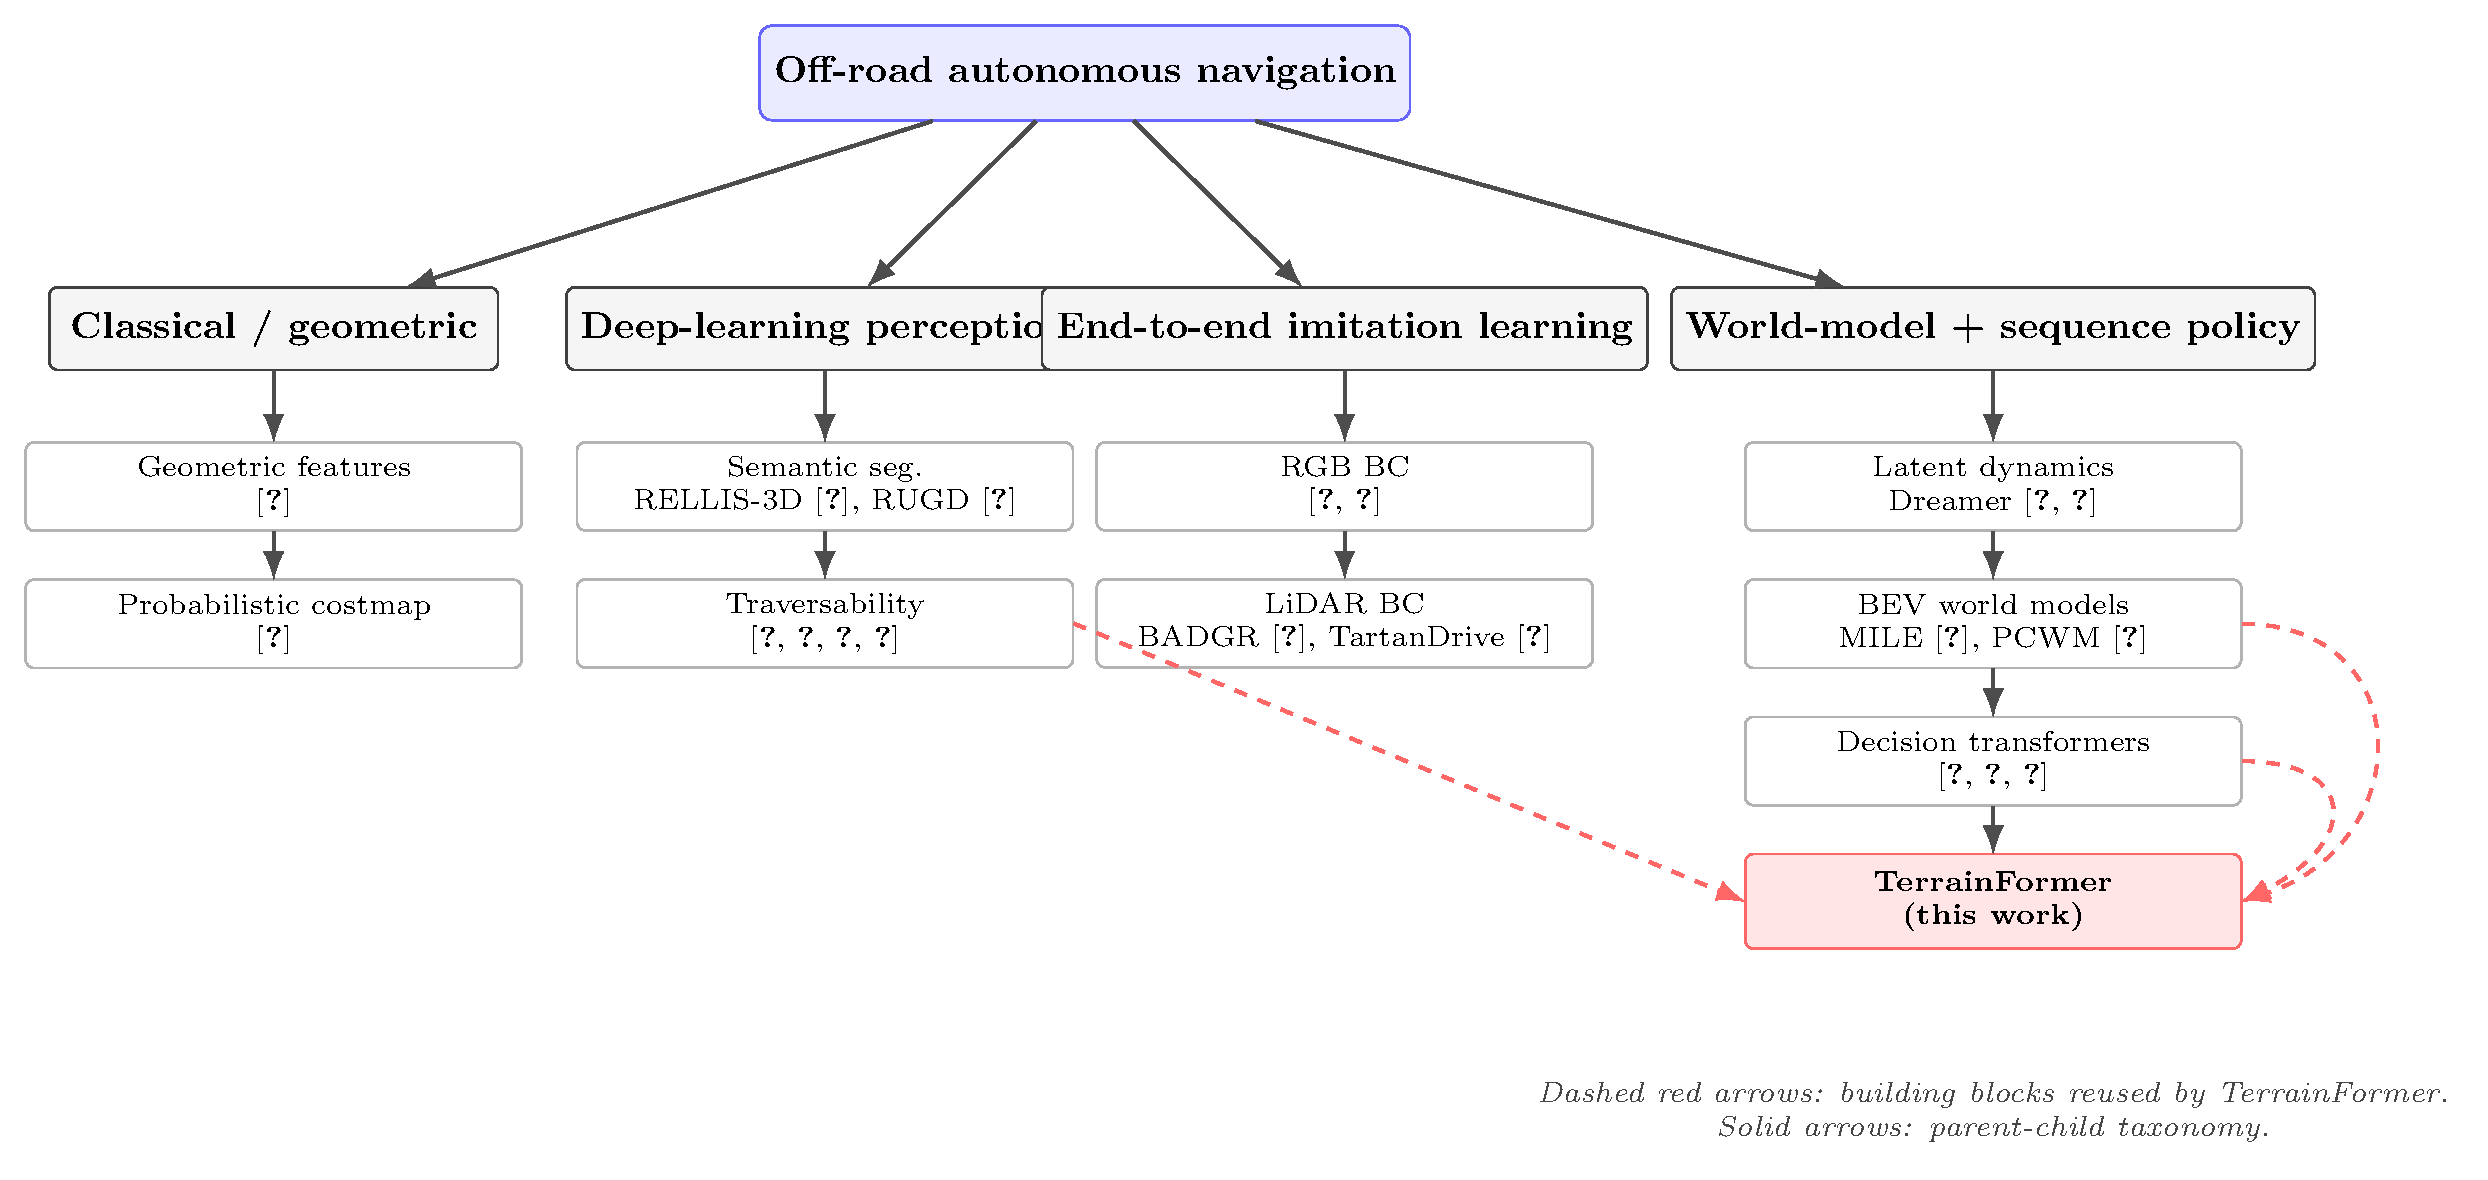
\includegraphics[width=\linewidth]{tech_tree.png}
    \caption{\DIFaddFL{Taxonomy of related work on off-road autonomous navigation. The four solid-line branches are classical geometric approaches, deep-learning perception (semantic segmentation and traversability), end-to-end imitation learning, and the more recent world-model-plus-sequence-policy family. TerrainFormer sits at the leaf of the last branch. Dashed red arrows mark the prior components TerrainFormer reuses: BEV world models from urban driving \mbox{%DIFAUXCMD
\cite{hu2022, yang2023}}\hskip0pt%DIFAUXCMD
, decision-transformer architectures from offline RL \mbox{%DIFAUXCMD
\cite{chen2021, zheng2022, janner2021}}\hskip0pt%DIFAUXCMD
, and self-supervised traversability/segmentation targets from deep-learning perception \mbox{%DIFAUXCMD
\cite{wellhausen2019, frey2023, castro2023}}\hskip0pt%DIFAUXCMD
.}}
    \label{fig:tech_tree}
\end{figure}

\DIFadd{Tables~\ref{tab:method_arch} and~\ref{tab:method_caps} compare TerrainFormer against representative systems on the architectural and methodological axes that drive their performance differences. Table~\ref{tab:method_arch} reports the architectural backbones (domain, perception, policy); Table~\ref{tab:method_caps} reports the deployment-relevant capabilities (action representation, cross-dataset training, real-time inference). The point of the comparison is not to claim TerrainFormer is uniformly better; several of the listed systems were designed for urban driving rather than off-road and use different action representations, sensor stacks, or training datasets. What the tables do show is which design choices are shared, which are specific to TerrainFormer, and where each design choice comes from in the literature.
}

\begin{table}[h]
\caption{\DIFaddFL{Methodological comparison, Part 1 of 2: architectural backbones. ``WM'' = world model with latent dynamics; ``DT'' = decision transformer (transformer-based sequence policy); ``E2E'' = direct sensors-to-action backbone without an intermediate latent.}}
\label{tab:method_arch}
\centering
\footnotesize
\begin{tabular}{lccc}
\toprule
\DIFaddFL{System }& \DIFaddFL{Domain }& \DIFaddFL{Perception }& \DIFaddFL{Policy }\\
\midrule
\DIFaddFL{BADGR \mbox{%DIFAUXCMD
\cite{kahn2021}              }\hskip0pt%DIFAUXCMD
}& \DIFaddFL{off-road  }& \DIFaddFL{RGB+IMU CNN          }& \DIFaddFL{E2E MLP        }\\
\DIFaddFL{TartanDrive \mbox{%DIFAUXCMD
\cite{triest2023}      }\hskip0pt%DIFAUXCMD
}& \DIFaddFL{off-road  }& \DIFaddFL{LiDAR+RGB+IMU        }& \DIFaddFL{E2E MLP        }\\
\DIFaddFL{Dreamer / DreamerV3 \mbox{%DIFAUXCMD
\cite{hafner2020,hafner2023} }\hskip0pt%DIFAUXCMD
}& \DIFaddFL{cont.\ control }& \DIFaddFL{RGB CNN        }& \DIFaddFL{WM imagination }\\
\DIFaddFL{MILE \mbox{%DIFAUXCMD
\cite{hu2022}                 }\hskip0pt%DIFAUXCMD
}& \DIFaddFL{urban     }& \DIFaddFL{camera $\to$ BEV     }& \DIFaddFL{WM + planner   }\\
\DIFaddFL{PCWM \mbox{%DIFAUXCMD
\cite{yang2023}               }\hskip0pt%DIFAUXCMD
}& \DIFaddFL{urban     }& \DIFaddFL{LiDAR point clouds   }& \DIFaddFL{WM             }\\
\DIFaddFL{Decision Transformer \mbox{%DIFAUXCMD
\cite{chen2021}}\hskip0pt%DIFAUXCMD
}& \DIFaddFL{offline RL}& \DIFaddFL{state vector         }& \DIFaddFL{DT             }\\
\DIFaddFL{Wayformer \mbox{%DIFAUXCMD
\cite{nayakanti2023}     }\hskip0pt%DIFAUXCMD
}& \DIFaddFL{urban     }& \DIFaddFL{multi-modal BEV      }& \DIFaddFL{transformer    }\\
\textbf{\DIFaddFL{TerrainFormer (ours)}}      & \textbf{\DIFaddFL{off-road}} & \textbf{\DIFaddFL{LiDAR $\to$ BEV (PointPillars)}} & \textbf{\DIFaddFL{WM + DT}} \\
\bottomrule
\end{tabular}
\end{table}

\begin{table}[h]
\caption{\DIFaddFL{Methodological comparison, Part 2 of 2: deployment-relevant capabilities. ``Cross-dataset'' = perception backbone is pretrained on data disjoint from the policy-training set. ``Real-time'' = end-to-end inference $\geq 10$\,FPS on a single GPU at the system's stated input size.}}
\label{tab:method_caps}
\centering
\footnotesize
\begin{tabular}{lccc}
\toprule
\DIFaddFL{System }& \DIFaddFL{Action repr. }& \DIFaddFL{Cross-dataset }& \DIFaddFL{Real-time }\\
\midrule
\DIFaddFL{BADGR \mbox{%DIFAUXCMD
\cite{kahn2021}              }\hskip0pt%DIFAUXCMD
}& \DIFaddFL{continuous       }& \DIFaddFL{---  }& \DIFaddFL{yes (10\,Hz) }\\
\DIFaddFL{TartanDrive \mbox{%DIFAUXCMD
\cite{triest2023}      }\hskip0pt%DIFAUXCMD
}& \DIFaddFL{continuous       }& \DIFaddFL{---  }& \DIFaddFL{yes (10\,Hz) }\\
\DIFaddFL{Dreamer / DreamerV3 \mbox{%DIFAUXCMD
\cite{hafner2020,hafner2023} }\hskip0pt%DIFAUXCMD
}& \DIFaddFL{continuous }& \DIFaddFL{no   }& \DIFaddFL{no (planning) }\\
\DIFaddFL{MILE \mbox{%DIFAUXCMD
\cite{hu2022}                 }\hskip0pt%DIFAUXCMD
}& \DIFaddFL{continuous traj. }& \DIFaddFL{no   }& \DIFaddFL{near (CARLA) }\\
\DIFaddFL{PCWM \mbox{%DIFAUXCMD
\cite{yang2023}               }\hskip0pt%DIFAUXCMD
}& \DIFaddFL{---              }& \DIFaddFL{no   }& \DIFaddFL{no }\\
\DIFaddFL{Decision Transformer \mbox{%DIFAUXCMD
\cite{chen2021}}\hskip0pt%DIFAUXCMD
}& \DIFaddFL{discrete        }& \DIFaddFL{---  }& \DIFaddFL{yes }\\
\DIFaddFL{Wayformer \mbox{%DIFAUXCMD
\cite{nayakanti2023}     }\hskip0pt%DIFAUXCMD
}& \DIFaddFL{continuous traj. }& \DIFaddFL{no   }& \DIFaddFL{yes }\\
\textbf{\DIFaddFL{TerrainFormer (ours)}}      & \textbf{\DIFaddFL{discrete (12 actions)}} & \textbf{\DIFaddFL{yes}} & \textbf{\DIFaddFL{yes ($\sim$50\,FPS)}} \\
\bottomrule
\end{tabular}
\end{table}

\DIFadd{Three observations of Tables~\ref{tab:method_arch} and~\ref{tab:method_caps} are note worthy. (i) BADGR \mbox{%DIFAUXCMD
\cite{kahn2021} }\hskip0pt%DIFAUXCMD
and TartanDrive \mbox{%DIFAUXCMD
\cite{triest2023} }\hskip0pt%DIFAUXCMD
are the closest off-road comparators, both end-to-end. Neither separates terrain representation from action selection, so the perception layer cannot be evaluated independently or transferred. TerrainFormer's two-phase split is what makes the cross-dataset measurement in Section~\ref{sec:results} possible at all. (ii) MILE \mbox{%DIFAUXCMD
\cite{hu2022} }\hskip0pt%DIFAUXCMD
and PCWM \mbox{%DIFAUXCMD
\cite{yang2023} }\hskip0pt%DIFAUXCMD
bring world-model machinery to urban driving with the same BEV-then-transformer pattern we use, but they consume a single urban dataset and output continuous trajectories. The architectural lineage is real but the off-road action vocabulary and cross-dataset protocol are new here. (iii) The original Decision Transformer \mbox{%DIFAUXCMD
\cite{chen2021} }\hskip0pt%DIFAUXCMD
treats policy learning as autoregressive sequence modelling but operates on state vectors, not perception. Pairing it with a BEV world model is the architectural step that turns it into a perception-aware policy.
}

\DIFaddend % ============================================================
\section{Methodology}
\label{sec:methodology}
% ============================================================

TerrainFormer comprises four principal components arranged in a hierarchical pipeline: (1) a LiDAR encoder that processes raw 3D point clouds into dense features, (2) a BEV projection module that creates spatial feature maps suitable for downstream processing, (3) a world model that learns terrain dynamics and latent representations through self-supervised pretraining, and (4) a temporal decision transformer that predicts discrete navigation actions conditioned on temporal context and automatically-derived goal directions. Training proceeds in two phases: self-supervised world model pretraining (Phase~1) using multi-dataset LiDAR observations, followed by behavio\DIFdelbegin \DIFdel{u}\DIFdelend ral cloning for the temporal decision transformer (Phase~2) on separated sequences.

Fig.~\ref{fig:architecture} gives the high-level dataflow at a glance: a point cloud (top) is encoded into a BEV feature map, compressed by the world model into 64 latent tokens, and finally consumed by the decision transformer to produce action chunks. To keep the high-level view readable, Fig.~\ref{fig:architecture} deliberately omits internal block details; expanded views of each component are provided in subsequent figures referenced from the relevant subsections: the PointPillars encoder in Fig.~\ref{fig:encoder_diagram} (Section~\ref{sec:lidar_encoder}), the world-model internals in Fig.~\ref{fig:world_model_diagram} (Section~\ref{sec:world_model}), and the decision-transformer token layout in Fig.~\ref{fig:dt_diagram} (Section~\ref{sec:decision_transformer}). The remainder of this section walks through the components in pipeline order, with each subsection describing one block of Fig.~\ref{fig:architecture}.

\begin{figure*}[!t]
    \centering
    % NOTE TO TYPESETTER: please supply a vector (PDF/SVG) version of this figure;
    % the current raster image becomes blurry at journal print resolution. Increase
    % all in-figure font sizes to ~9pt minimum so that text remains readable when
    % the figure is reduced to single-column width.
    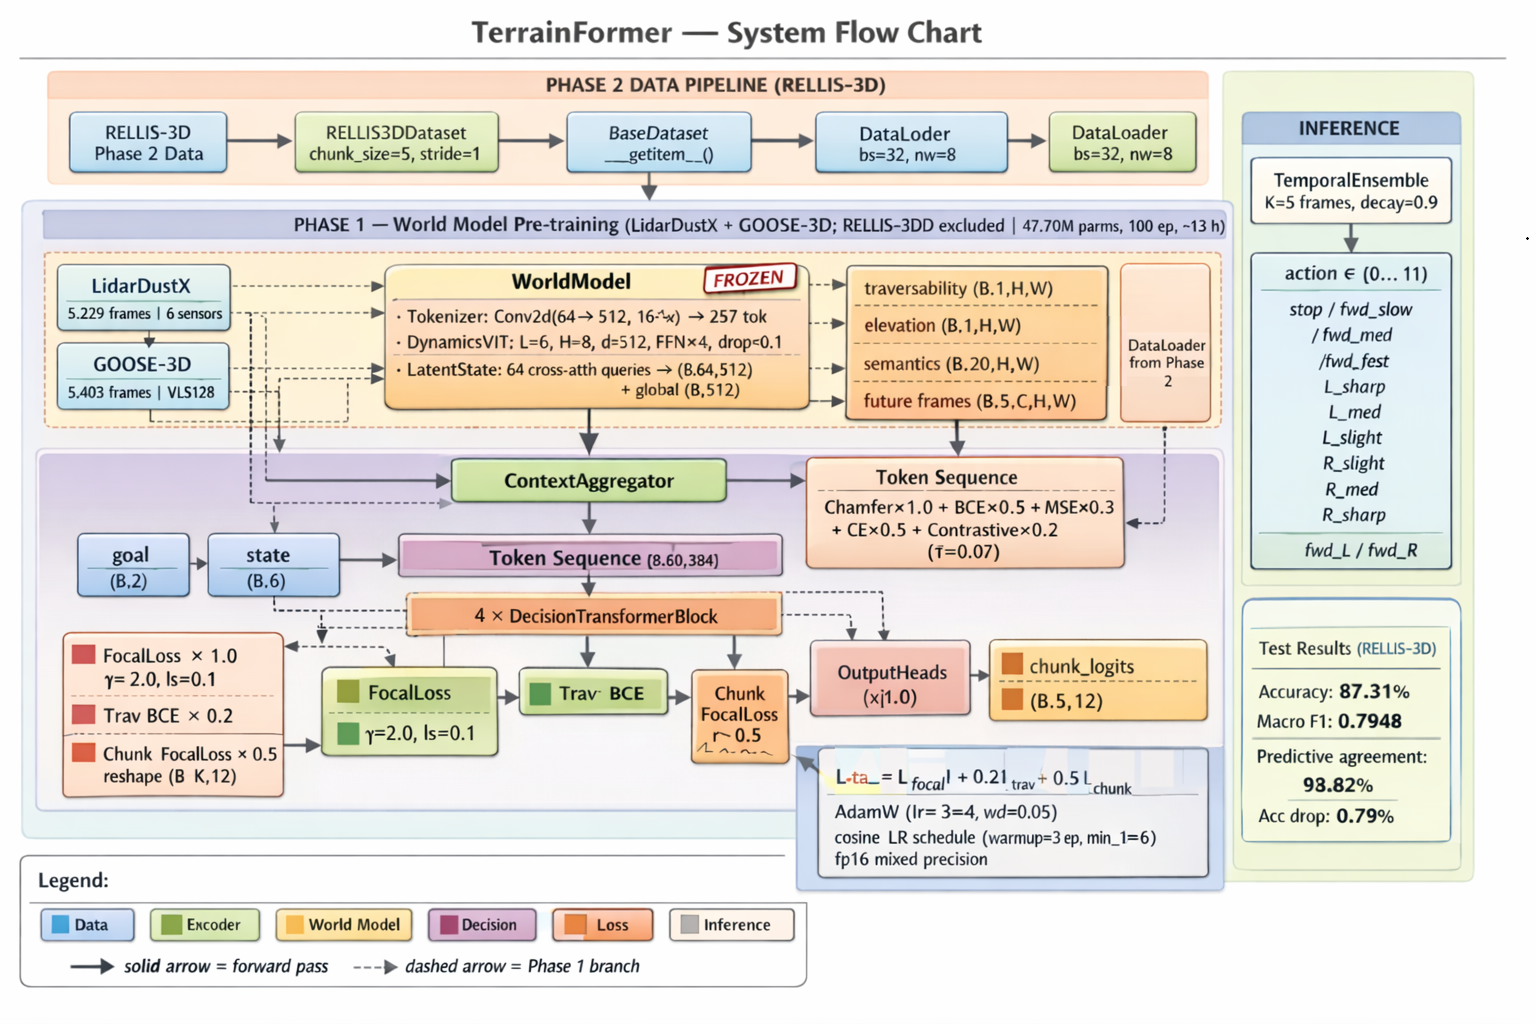
\includegraphics[width=\linewidth]{terrainformer_flowchart.png}
    \caption{%
        High-level dataflow of TerrainFormer. A raw LiDAR point cloud (left) passes through the PointPillars encoder to a BEV feature map, which the world model compresses to 64 latent tokens; the decision transformer attends jointly to these tokens, an action-history buffer, and a learnable chunk query, and predicts $K{=}5$ future actions. \DIFdelbeginFL \DIFdelFL{TemporalEnsemble }\DIFdelendFL \DIFaddbeginFL \DIFaddFL{temporal prediction aggregation }\DIFaddendFL (right) averages overlapping chunks for jitter-free outputs. \textbf{Block-internal details are deliberately omitted here} and are shown in expanded views: encoder (Fig.~\ref{fig:encoder_diagram}), world model (Fig.~\ref{fig:world_model_diagram}), and decision transformer (Fig.~\ref{fig:dt_diagram}). Symbol legend: $B$ batch, $N$ points/scan, $H{\times}W{=}256{\times}256$ BEV cells, $d{=}512$ embedding, $K{=}5$ chunk, $A{=}12$ actions.
    }
    \label{fig:architecture}
\end{figure*}

\subsection{LiDAR Encoder}
\label{sec:lidar_encoder}

The LiDAR encoder processes raw 3D point clouds of up to $N = 65{,}536$ points, where each point has four features $(x, y, z, i)$ representing spatial coordinates and intensity. We employ a PointPillars-based encoder \cite{lang2019} that directly converts point clouds to BEV features, chosen for its architectural alignment with our BEV-centric pipeline and real-time performance characteristics. Fig.~\ref{fig:encoder_diagram} shows the encoder in isolation, with each pipeline stage labelled.

\begin{figure}[H]
    \centering
    \DIFdelbeginFL %DIFDELCMD < 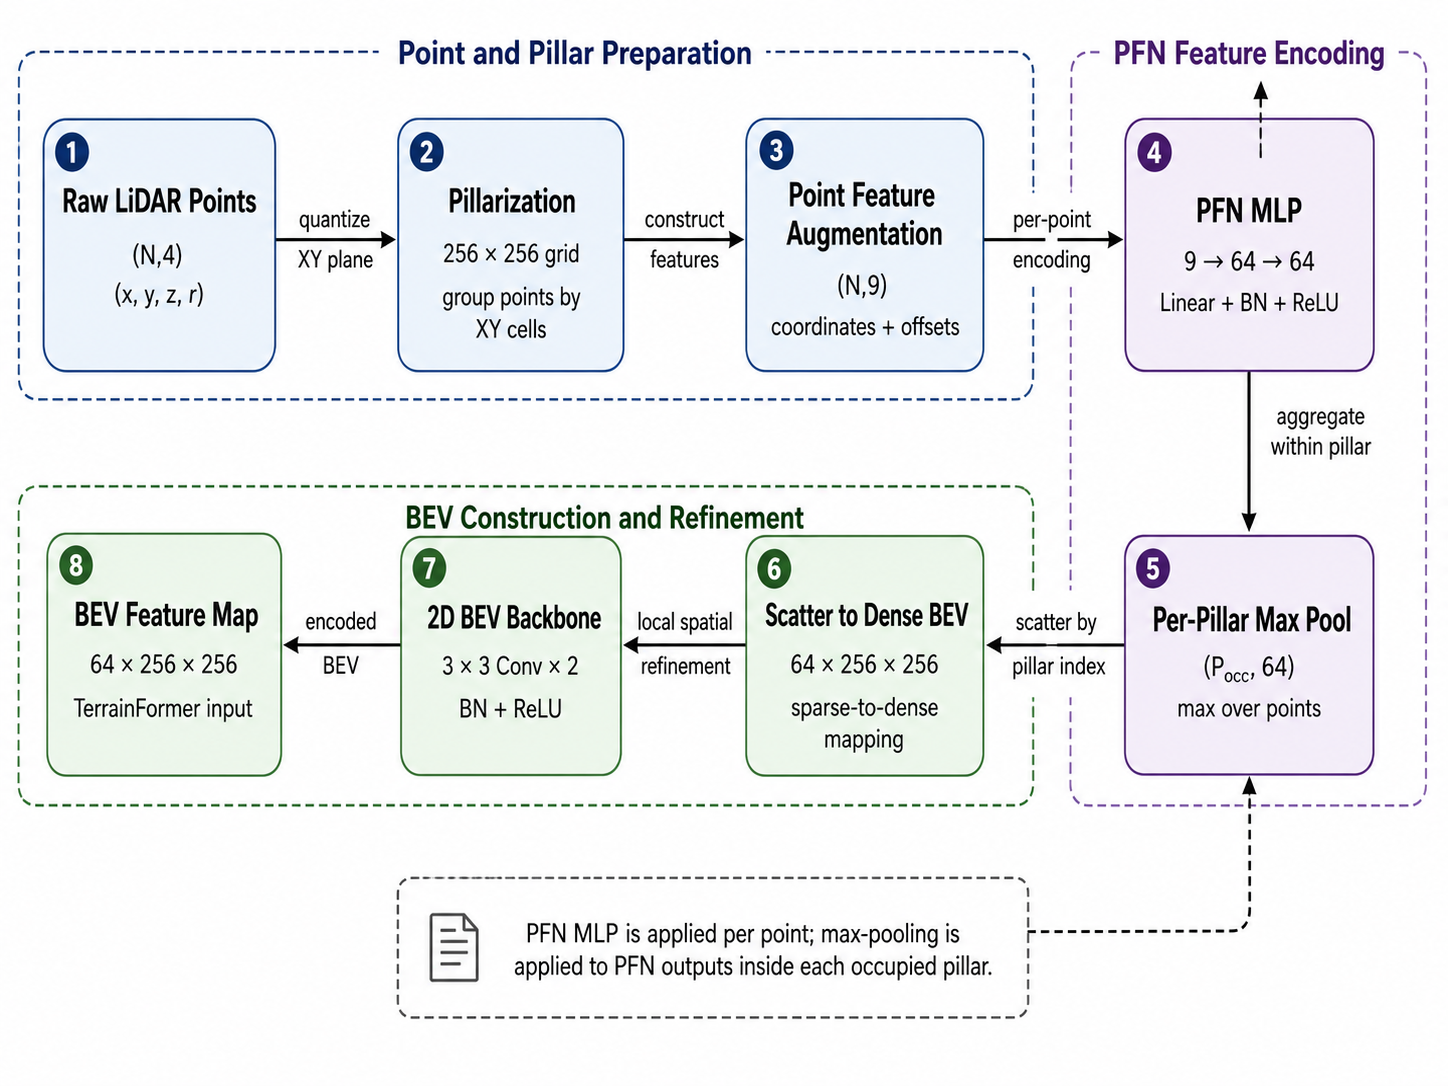
\includegraphics[width=\linewidth]{encoder_diagram.pdf}
%DIFDELCMD <     %%%
\DIFdelendFL \DIFaddbeginFL 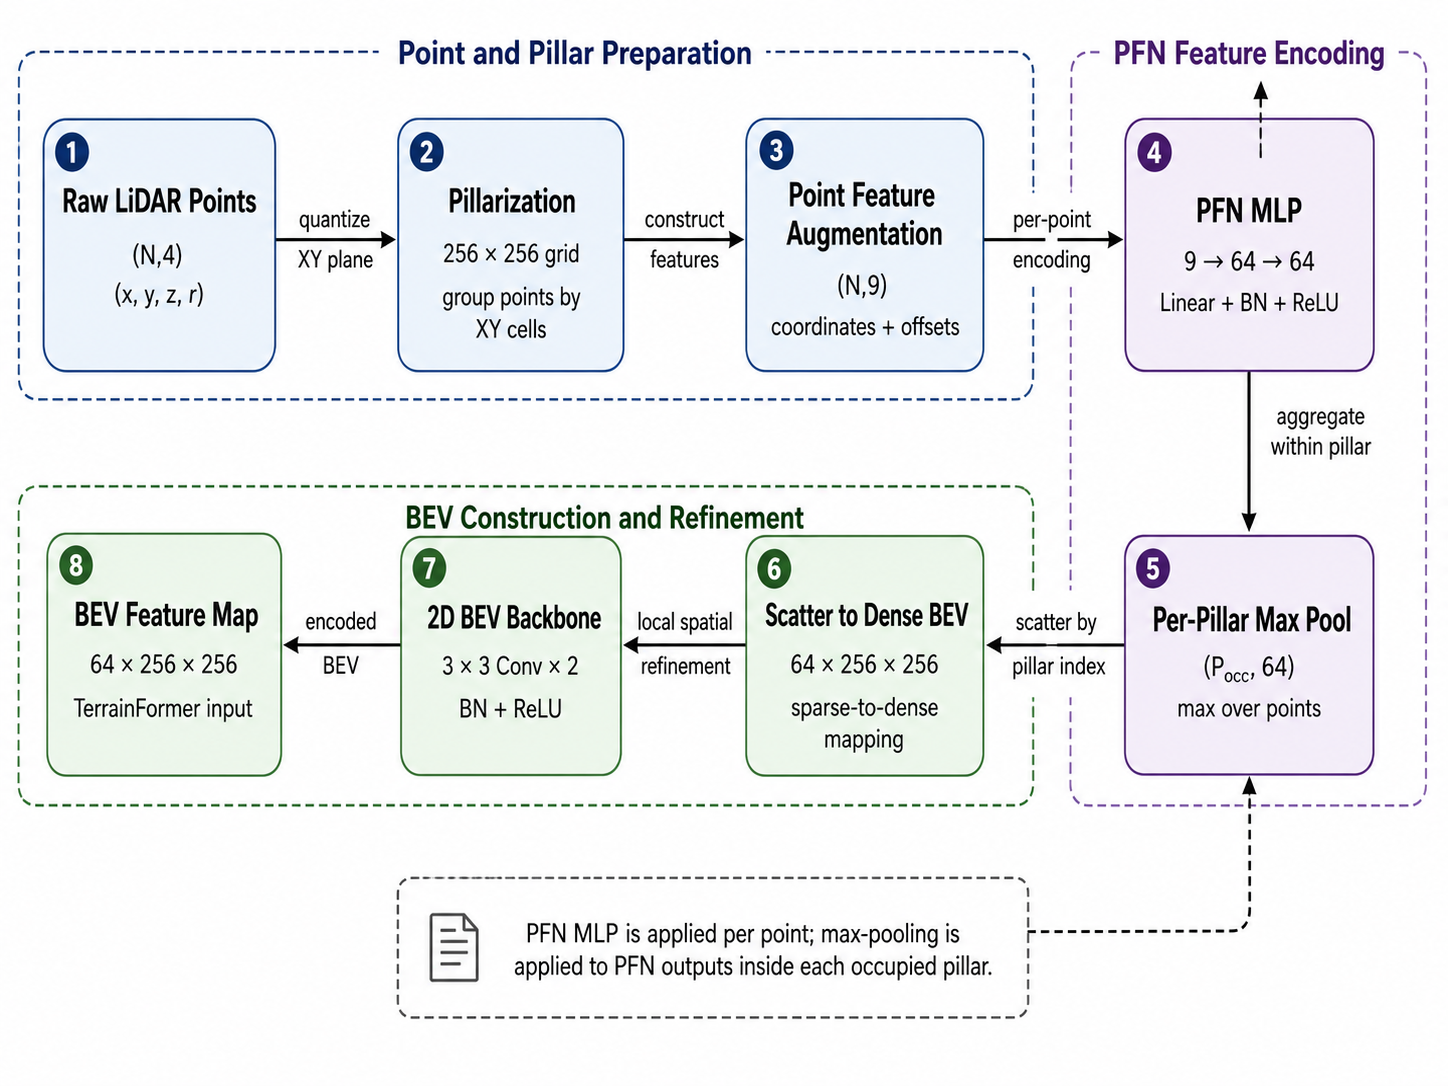
\includegraphics[width=\linewidth]{encoder_diagram.png}
    \DIFaddendFL \caption{\textcolor{red}{Component view of the PointPillars LiDAR encoder used by TerrainFormer. The pipeline is read left-to-right (top row) then folded back right-to-left (bottom row). Critically, the per-point MLP operates independently on every point and is \emph{not} pooled itself; max-pooling is applied to the MLP \emph{outputs} within each pillar (Section~\ref{sec:lidar_encoder}). Tensor shapes are annotated below each block.}}
    \label{fig:encoder_diagram}
\end{figure}

\subsubsection{PointPillars Architecture}
The encoder operates as follows:

\begin{enumerate}
    \item \textbf{Pillarization}: Points are discretized into vertical pillars on a $256 \times 256$ BEV grid covering $100\,\text{m} \times 100\,\text{m}$ ($x, y \in [-50, 50]$\,m). Each pillar aggregates up to 32 points; pillars exceeding this cap are uniformly subsampled.
    \item \textbf{Feature Augmentation}: Each point is augmented with 5 additional features: $(x_c, y_c, z_c)$ offset from pillar centroid and $(x_p, y_p)$ offset from pillar geometric center, yielding a 9-dimensional per-point input.
    \item \textbf{Pillar Feature Network}: A two-layer pointwise MLP ($9 \rightarrow 64 \rightarrow 64$ with BatchNorm and ReLU) is applied independently to every point. The MLP itself is \emph{not} pooled; rather, the per-point 64-dimensional outputs are subsequently aggregated within each pillar by an element-wise max operation (implemented via vectorized \texttt{scatter\_reduce}). The result is a single 64-dimensional feature per occupied pillar, which is then scattered back onto the $256 \times 256$ BEV grid (empty cells set to zero).
    \item \textbf{BEV Backbone}: Two $3 \times 3$ convolutional layers with BatchNorm and ReLU refine the resulting $64 \times 256 \times 256$ spatial feature map.
\end{enumerate}

The PointPillars encoder achieves ${\sim}5$\,ms latency on a single NVIDIA Quadro RTX 8000 desktop GPU\footnote{All latency numbers in this paper were measured on the same workstation: an NVIDIA Quadro RTX 8000 (48\,GB GDDR6 VRAM, Turing TU102 architecture) with an Intel Core i9 CPU and 64\,GB RAM, running PyTorch 2.1 with FP16 inference. Each value is the mean over 1{,}000 inference passes after a 100-pass warm-up; standard deviations were below 0.4\,ms in all cases.}, enabling real-time inference at 10\,Hz LiDAR rates with ample margin for downstream processing.

\subsubsection{Encoder Design Rationale}
We considered alternative architectures including PointNet++ \cite{qi2017b}, which offers hierarchical set abstraction for fine-grained local geometry learning. However, PointPillars was selected for three reasons: (1) \textbf{architectural alignment}---PointPillars produces BEV features directly, matching the world model's expected input without intermediate projection layers; (2) \textbf{latency}---PointPillars achieves $5\times$ lower encoder latency, critical for real-time navigation at 10\,Hz; (3) \textbf{compensating capacity}---the 6-layer Dynamics Transformer provides sufficient representational capacity to learn fine-grained terrain patterns that hierarchical point encoders would capture at the encoder level.

Table~\ref{tab:encoder_comparison} compares the two encoder architectures, including per-component FPS. PointPillars achieves ${\sim}200$\,FPS at the encoder stage (vs.\ ${\sim}40$\,FPS for PointNet++), and the full TerrainFormer pipeline runs at ${\sim}50$\,FPS end-to-end. A hypothetical PointNet++ variant would achieve only ${\sim}25$\,FPS end-to-end, falling below the 30\,FPS threshold required for responsive real-time navigation and exceeding the 100\,ms frame budget when combined with downstream processing.

\begin{table}[h]
\caption{LiDAR Encoder Comparison: PointPillars (Ours) vs.\ PointNet++}
\label{tab:encoder_comparison}
\centering
\begin{tabular}{lcc}
\toprule
Metric & PointPillars (Ours) & PointNet++ \\
\midrule
Encoder latency   & ${\sim}5$\,ms          & ${\sim}25$\,ms \\
Encoder FPS       & ${\sim}200$\,FPS       & ${\sim}40$\,FPS \\
Full-system FPS   & ${\sim}50$\,FPS        & ${\sim}25$\,FPS \\
Parameters        & 0.15\,M                & 1.48\,M \\
Output format     & BEV (direct)           & Point features \\
BEV projection    & Built-in               & Requires additional \\
TensorRT support  & Full                   & Limited \\
Real-time (10\,Hz) & \checkmark            & $\times$ \\
\bottomrule
\end{tabular}
\smallskip
\parbox{\columnwidth}{\footnotesize Full-system FPS computed as $1000\,\text{ms}\,/\,(t_\text{enc}+10+5)$, where $10$\,ms and $5$\,ms are the world model and decision transformer latencies respectively.}
\end{table}

The $5\times$ latency advantage of PointPillars (${\sim}5$\,ms vs.\ ${\sim}25$\,ms) arises from three distinct architectural factors, not simply from parameter count (PointPillars has ${\sim}10\times$ \emph{fewer} parameters, but parameter count alone does not explain the wall-clock gap):

\begin{enumerate}
    \item \textbf{Memory layout (dominant factor)}: PointPillars produces a regular, dense $256{\times}256$ BEV tensor in a single \texttt{scatter\_reduce} call, which maps directly onto GPU memory-coalescing hardware. PointNet++ instead performs iterative neighborhood queries (\texttt{ball\_query}, \texttt{KNN}) on irregular point sets; these are scattered memory accesses with low cache-line utilisation and high index-arithmetic overhead.
\textcolor{red}{    \item \textbf{Hierarchy depth}: PointNet++ stacks 3--4 set-abstraction layers, each requiring its own grouping operation. PointPillars groups points exactly once (during \DIFdelbegin \DIFdel{pillarisation}\DIFdelend \DIFaddbegin \DIFadd{pillarization}\DIFaddend ) and runs the remaining layers as standard 2D convolutions, which cuDNN already has fast kernels for.}
    \item \textbf{Output-format alignment}: PointPillars produces BEV features natively; the downstream ViT world model can consume them without an intermediate projection step. A PointNet++ variant would require an additional point-to-BEV \DIFdelbegin \DIFdel{rasterisation }\DIFdelend \DIFaddbegin \DIFadd{rasterization }\DIFaddend layer (\textasciitilde2\,ms in our profiling), which the table does not separately charge to its column.
\end{enumerate}

These factors compound: even with TensorRT \DIFdelbegin \DIFdel{optimisation}\DIFdelend \DIFaddbegin \DIFadd{optimization}\DIFaddend , PointNet++ remains ${\sim}3\times$ slower than PointPillars in our profiling. Empirically, for BEV-based downstream tasks, PointPillars consistently matches PointNet++ performance on established benchmarks while enabling TensorRT \DIFdelbegin \DIFdel{optimisation }\DIFdelend \DIFaddbegin \DIFadd{optimization }\DIFaddend for embedded deployment, which is critical for the real-time off-road navigation setting where rapid terrain changes and dynamic obstacles demand a low-latency perception-to-action pipeline.

\subsubsection{BEV Output}
The encoder produces a BEV feature map $\mathbf{F}_\text{BEV} \in \mathbb{R}^{64 \times 256 \times 256}$ and a global feature vector $\mathbf{z}_\text{encoder} \in \mathbb{R}^{1024}$ via adaptive pooling followed by linear projection.

\subsection{World Model}
\label{sec:world_model}

The world model learns to predict terrain dynamics and extract rich representations from BEV features through self-supervised pretraining. It consists of three components: a terrain tokenizer, a dynamics transformer, and a latent state module. Fig.~\ref{fig:world_model_diagram} shows the three components in sequence together with the four self-supervised prediction heads.

\begin{figure}[H]
    \centering
    \DIFdelbeginFL %DIFDELCMD < 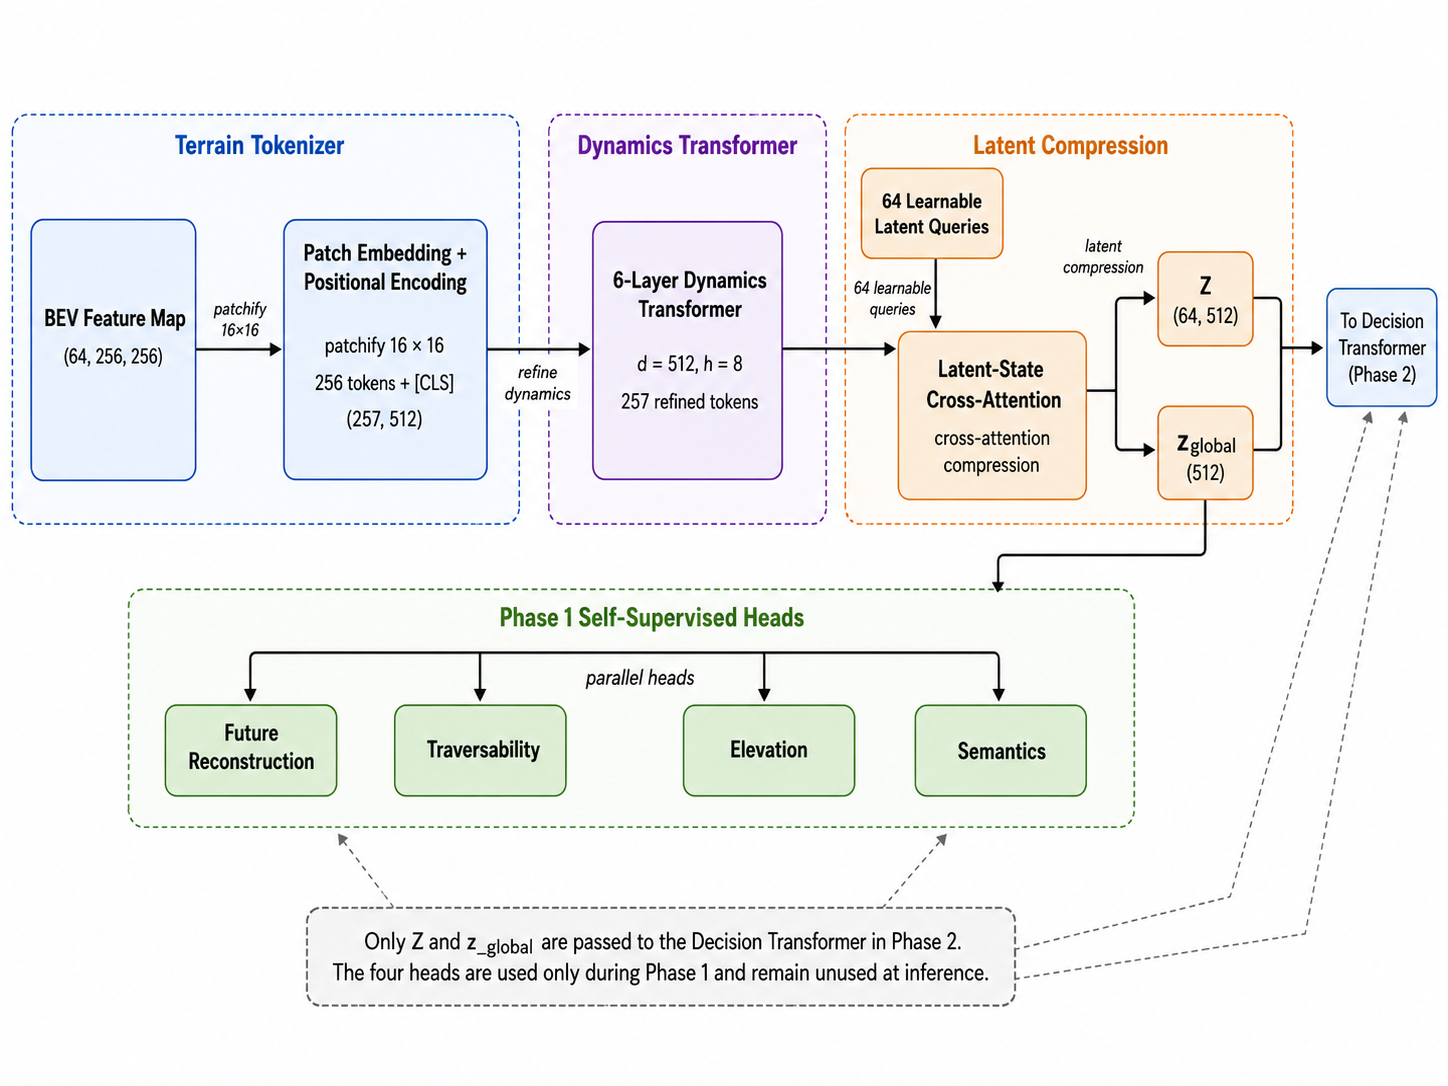
\includegraphics[width=\linewidth]{world_model_diagram.pdf}
%DIFDELCMD <     %%%
\DIFdelendFL \DIFaddbeginFL 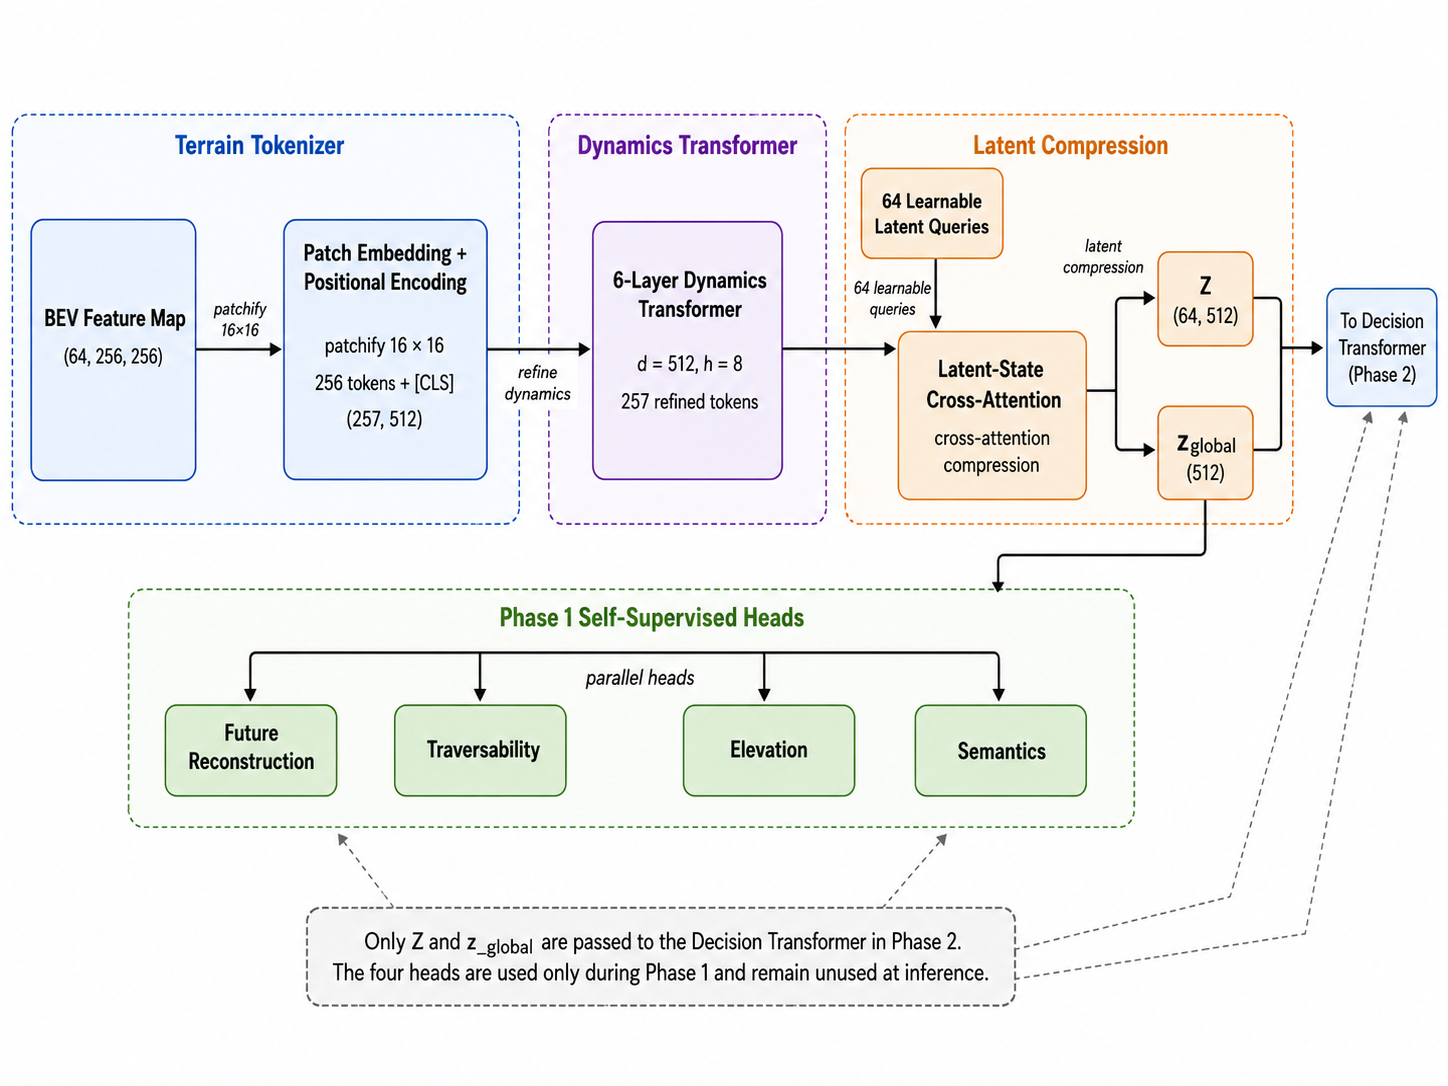
\includegraphics[width=\linewidth]{world_model_diagram.png}
    \DIFaddendFL \caption{\textcolor{red}{Component view of the world model. The three internal modules (terrain tokenizer, dynamics transformer, latent compression) and the four self-supervised heads used during Phase 1 pretraining are shown explicitly. Only $\mathbf{Z}$ (64 latent tokens) and $\mathbf{z}_\text{global}$ are passed on to the decision transformer in Phase 2; the four prediction heads remain unused at inference and after Phase 1 the entire world model is frozen.}}
    \label{fig:world_model_diagram}
\end{figure}

\subsubsection{Terrain Tokenizer}
The BEV feature map $\mathbf{F}_\text{BEV}$ is divided into non-overlapping patches of size $16 \times 16$ pixels, yielding $P = (256/16)^2 = 256$ patches. Each patch is projected to a token of dimension $d = 512$ via a convolutional embedding layer. Learned positional encodings $\mathbf{E}_\text{pos} \in \mathbb{R}^{256 \times 512}$ and a learnable \texttt{[CLS]} token are prepended, producing an input sequence of $257$ tokens.

\subsubsection{Dynamics Transformer}
The token sequence is processed by a 6-layer transformer encoder with the following configuration per layer: $d_\text{model} = 512$, $h = 8$ attention heads, head dimension $d_k = 64$, MLP ratio $4\times$ (intermediate dimension $2048$), and dropout rate $0.1$. The architecture uses pre-norm (LayerNorm before attention and MLP) following the convention of Vision Transformers \cite{dosovitskiy2021}.

\subsubsection{Latent State Compression}
To produce a compact representation for the decision transformer, we employ a cross-attention-based compression module. A set of $64$ learnable latent queries $\mathbf{Q}_\text{latent} \in \mathbb{R}^{64 \times 512}$ attend to the $257$ transformer output tokens via multi-head cross-attention ($h = 8$ heads), producing compressed latent tokens $\mathbf{Z} \in \mathbb{R}^{64 \times 512}$. A global feature vector $\mathbf{z}_\text{global} \in \mathbb{R}^{512}$ is obtained via mean pooling over the latent tokens followed by a linear projection.

\subsubsection{Prediction Heads}
Four parallel prediction heads decode the latent representations for self-supervised training:

\begin{enumerate}
    \item \textbf{Future Reconstruction}: Predicts the next 5 frames' BEV features at patch resolution, output $\mathbb{R}^{5 \times 64 \times 16 \times 16}$.
    \item \textbf{Traversability}: Transposed convolution upsampling ($4\times$) to produce a binary traversability map $\mathbb{R}^{1 \times 256 \times 256}$ with sigmoid activation.
    \item \textbf{Elevation}: Same architecture, predicting continuous elevation values $\mathbb{R}^{1 \times 256 \times 256}$.
    \item \textbf{Semantics}: Transposed convolution upsampling to produce per-class logits $\mathbb{R}^{C \times 256 \times 256}$ where $C = 20$ for RELLIS-3D semantic classes.
\end{enumerate}

\subsection{Decision Transformer}
\label{sec:decision_transformer}

The decision transformer predicts discrete navigation actions using a token-sequence architecture that provides full cross-attention between spatial world features, temporal action history, and learnable future-action query tokens. The token layout and output heads are illustrated in Fig.~\ref{fig:dt_diagram}.

\begin{figure*}[!t]
    \centering
    \DIFdelbeginFL %DIFDELCMD < 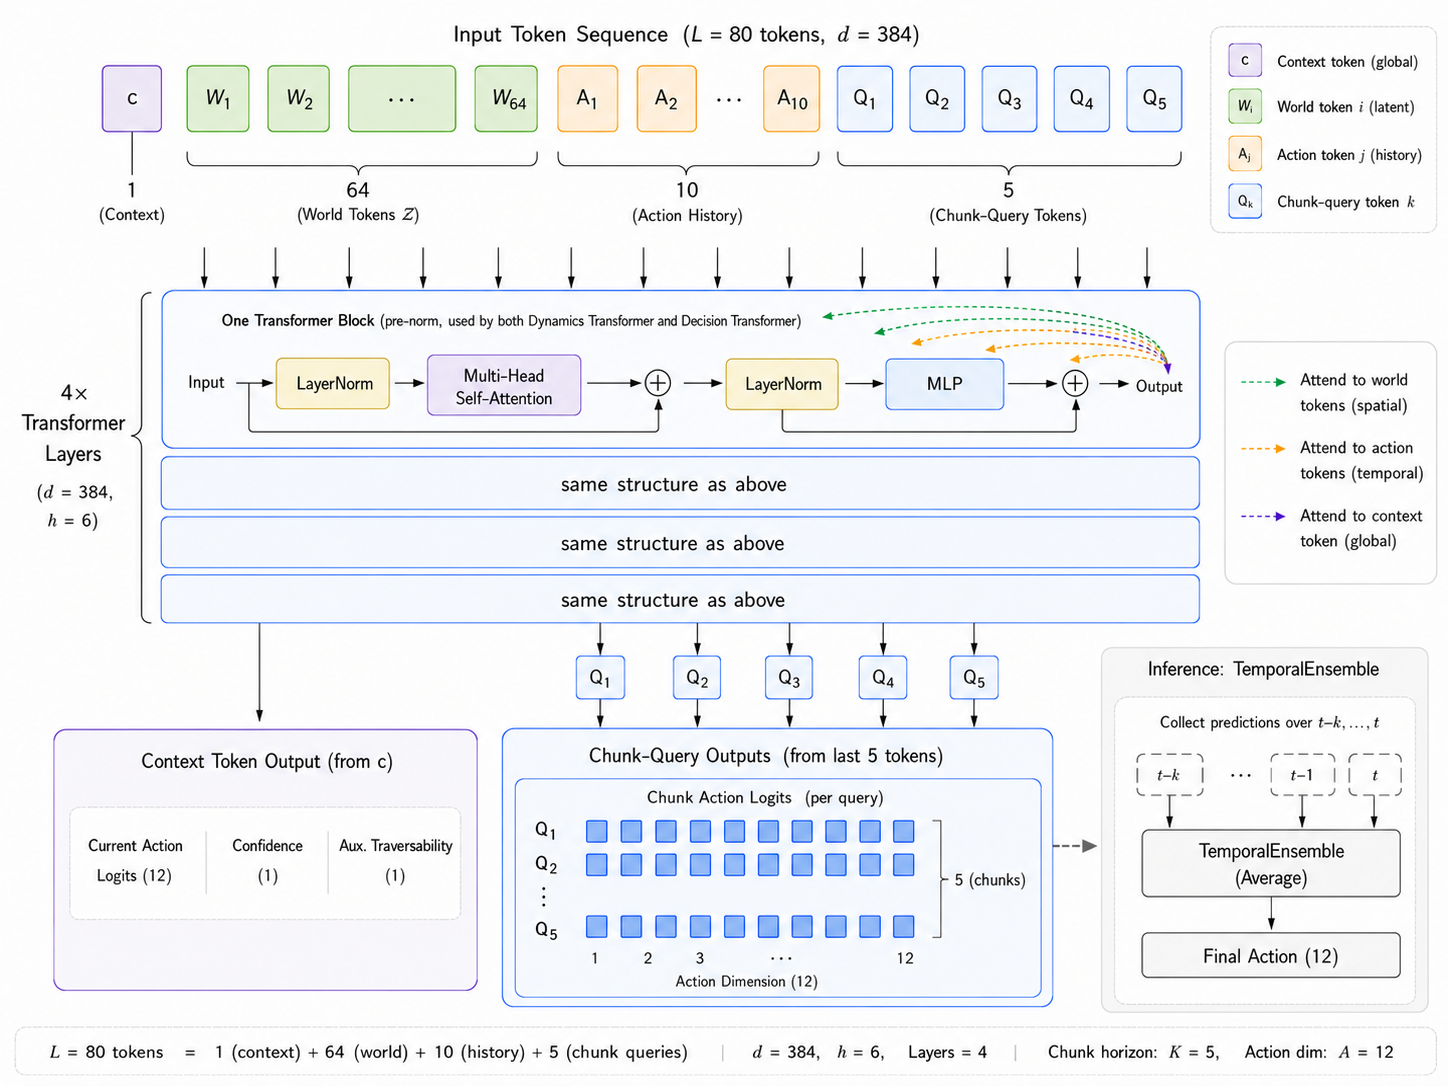
\includegraphics[width=\linewidth]{dt_diagram.pdf}
%DIFDELCMD <     %%%
\DIFdelendFL \DIFaddbeginFL 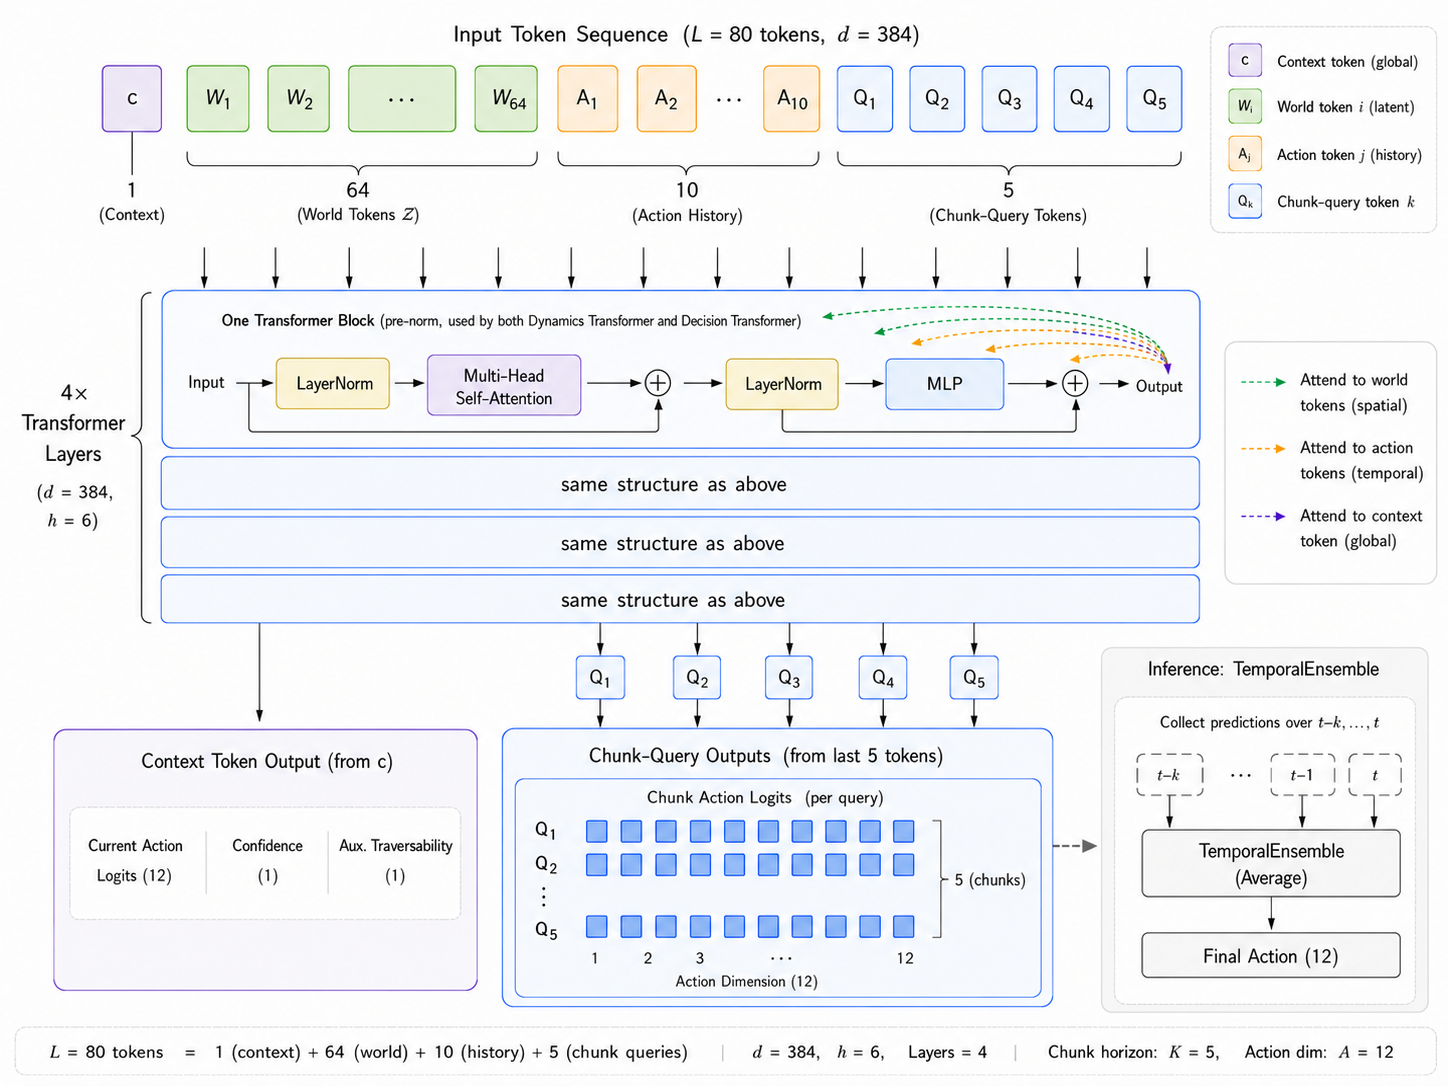
\includegraphics[width=\linewidth]{dt_diagram.png}
    \DIFaddendFL \caption{\textcolor{red}{Component view of the decision transformer. The 80-token sequence (top) is composed of one context token $\mathbf{c}$, the 64 world latent tokens, 10 action-history tokens, and 5 learnable chunk-query tokens. Dashed red arrows from one chunk query illustrate the cross-modal attention pattern: every chunk query attends to all spatial (world) and temporal (action-history) tokens simultaneously. The context-token output predicts the current action and confidence; the last five output positions predict the action chunk $(B, K{=}5, A{=}12)$; \DIFdelbeginFL \DIFdelFL{TemporalEnsemble }\DIFdelendFL \DIFaddbeginFL \DIFaddFL{temporal prediction aggregation }\DIFaddendFL at inference aggregates overlapping chunks with exponential-decay weighting.}}
    \label{fig:dt_diagram}
\end{figure*}

\subsubsection{Token Sequence Architecture}
Inspired by action chunking~\cite{zhao2023act}, the model simultaneously predicts the next $K{=}5$ actions per frame rather than a single step, improving temporal coherence and enabling anticipatory look-ahead. The transformer processes a fixed-length sequence of $L{=}80$ tokens:
\begin{equation}
    \mathbf{X} = \bigl[\mathbf{c};\;\mathbf{W}_{1:64};\;\mathbf{A}_{1:10};\;\mathbf{Q}_{1:5}\bigr]
    \;\in \mathbb{R}^{80 \times 384}
\end{equation}
where $\mathbf{c} \in \mathbb{R}^{384}$ is a fused \emph{context token}, $\mathbf{W}_{1:64}$ are projected world latent tokens (BEV spatial features), $\mathbf{A}_{1:10}$ are per-step action history embeddings (temporal features), and $\mathbf{Q}_{1:5}$ are $K$ learnable \emph{chunk query} tokens that represent the $K$ future action predictions.

Learnable positional embeddings $\mathbf{E}_\text{pos} \in \mathbb{R}^{80 \times 384}$ are added to the full sequence to encode token order.

\subsubsection{Context Aggregator}
The context token $\mathbf{c}$ fuses four information sources through a two-layer MLP followed by cross-attention over the world latent tokens $\mathbf{Z}$:
\begin{itemize}
    \item \textbf{World global feature}: $\mathbf{z}_\text{global} \in \mathbb{R}^{512}$, linearly projected to $\mathbb{R}^{384}$.
    \item \textbf{Vehicle state}: $\mathbf{s} \in \mathbb{R}^{6}$ encoding velocity $(v_x, v_y)$, angular velocity $\omega$, and orientation (pitch, roll, yaw).
    \item \textbf{Goal direction}: $\mathbf{g} \in \mathbb{R}^{2}$ (Section~\ref{sec:goal_direction}).
    \item \textbf{Action aggregate}: $\mathbf{e}_a \in \mathbb{R}^{128}$, mean-pooled over 10 per-step action embeddings.
\end{itemize}
\begin{equation}
    \mathbf{c} = \text{CrossAttn}\!\left(\text{MLP}_\text{fuse}([\text{proj}(\mathbf{z}_\text{global}); \mathbf{e}_s; \mathbf{e}_g; \mathbf{e}_a]),\;\mathbf{Z}\right) \in \mathbb{R}^{384}
\end{equation}

\subsubsection{Token Projections}
World latent tokens $\mathbf{Z} \in \mathbb{R}^{64 \times 512}$ are projected to $\mathbb{R}^{64 \times 384}$ via a linear layer. Action history embeddings are produced per-step (preserving temporal structure) and projected to $\mathbb{R}^{10 \times 384}$ via a separate linear layer. Chunk queries $\mathbf{Q} \in \mathbb{R}^{5 \times 384}$ are learnable parameters initialized with truncated-normal distribution ($\sigma{=}0.02$).

\subsubsection{Transformer Backbone}
The 80-token sequence is processed by a 4-layer transformer with $d_\text{model}{=}384$, $h{=}6$ attention heads, head dimension $d_k{=}64$, MLP ratio $4\times$, and dropout $0.1$, using pre-norm (LayerNorm before attention and MLP). Full self-attention over all 80 tokens enables each chunk query to attend simultaneously to BEV spatial context (world tokens) and temporal action history (action tokens), providing richer conditioning than single-token architectures.

\subsubsection{Output Heads}
\begin{enumerate}
    \item \textbf{Current-step action}: The context token output $\mathbf{x}_0 \in \mathbb{R}^{384}$ is decoded by an action head (MLP $384{\to}12$), a confidence head (MLP $384{\to}1$ with sigmoid), and an auxiliary traversability head (MLP $384{\to}1$ with sigmoid).
    \item \textbf{Action chunk}: Each of the last $K{=}5$ output tokens $\mathbf{x}_{-5:} \in \mathbb{R}^{5 \times 384}$ is independently decoded by the shared action head, yielding chunk logits $\in \mathbb{R}^{K \times 12}$.
\end{enumerate}

\subsubsection{Temporal Ensembling at Inference}
At inference, each frame produces a $K{=}5$ action chunk. Overlapping chunks from the last $K$ consecutive frames are aggregated via \emph{\DIFdelbegin \DIFdel{TemporalEnsemble}\DIFdelend \DIFaddbegin \DIFadd{temporal prediction aggregation}\DIFaddend }~\cite{zhao2023act} using exponential-decay weighting:
\begin{equation}
    \hat{a}_t = \arg\max_a \;\frac{\displaystyle\sum_{k=0}^{K-1} \lambda^k \cdot \text{chunk}_{t-k}[k]}{\displaystyle\sum_{k=0}^{K-1} \lambda^k},
    \quad \lambda = 0.9
\end{equation}
where $\text{chunk}_{t-k}[k]$ is the $k$-th step prediction from the chunk generated $k$ frames ago. More recent predictions receive higher weight. This averaging suppresses prediction jitter and smooths action transitions without latency overhead.

\subsection{Action Space}
\label{sec:action_space}

We define a discrete action space of 12 forward-motion actions that combines speed and steering commands, derived from continuous vehicle poses via velocity and turn-rate thresholding (Table~\ref{tab:action_space}). The action space is designed specifically for forward-only driving scenarios characteristic of the RELLIS-3D dataset, which contains no backward motion. Actions are classified using a turn-first approach: turn rate magnitude determines the action category, with forward-speed actions reserved for minimal-turn scenarios.

\begin{table}[h]
\caption{Discrete Action Space (12 Forward-Motion Actions)}
\label{tab:action_space}
\centering
\begin{tabular}{clcl}
\toprule
ID & Action & ID & Action \\
\midrule
0 & Stop & 6 & Left slight \\
1 & Forward slow & 7 & Right slight \\
2 & Forward medium & 8 & Right medium \\
3 & Forward fast & 9 & Right sharp \\
4 & Left sharp & 10 & Forward left \\
5 & Left medium & 11 & Forward right \\
\bottomrule
\end{tabular}
\end{table}

Action labels are derived from ground-truth pose sequences by computing linear velocity and turn rate between consecutive frames ($\Delta t = 0.1$\,s). Using a turn-first classification approach, turn rate magnitude is evaluated first: sharp ($|\omega| \geq 0.6$ rad/s), medium ($0.3$--$0.6$), slight ($0.1$--$0.3$), or minimal ($< 0.1$). Turn actions (4--9) are assigned regardless of velocity; forward-speed actions (0--3) apply only when $|\omega| < 0.1$. Combined actions (10--11) represent fast forward motion ($v \geq 1.0$ m/s) with sharp turning. Since RELLIS-3D contains exclusively forward driving trajectories (no backward motion), the action space excludes backward-related actions, simplifying the classification task while maintaining expressiveness for off-road navigation.

\subsection{Goal Direction Computation}
\label{sec:goal_direction}

A critical component of directionally-conditioned navigation is the goal direction input, which informs the model where the vehicle should navigate. Rather than relying on externally-provided waypoints, we compute goal directions automatically from the vehicle's future trajectory encoded in the pose sequence.

For each frame $t$, the goal direction $\mathbf{g}_t \in \mathbb{R}^2$ is computed as the normalized displacement vector from the current position to a future position (lookahead $k=5$ frames), expressed in the vehicle's local coordinate frame:

\begin{equation}
    \mathbf{d}_t = \mathbf{p}_{t+k} - \mathbf{p}_t
\end{equation}
\begin{equation}
    \mathbf{g}_t = \mathbf{R}(-\psi_t) \cdot \frac{\mathbf{d}_t}{\|\mathbf{d}_t\|}
\end{equation}

where $\mathbf{p}_t = (x_t, y_t)$ is the vehicle position at frame $t$, $\psi_t$ is the yaw angle extracted from the rotation matrix, and $\mathbf{R}(-\psi_t)$ is the 2D rotation matrix that transforms world coordinates to the vehicle's local frame. This transformation ensures that $\mathbf{g}_t = (g_x, g_y)$ represents the goal direction relative to the vehicle's heading:
\begin{itemize}
    \item $g_x > 0$: goal is ahead of the vehicle
    \item $g_y > 0$: goal is to the left of the vehicle
    \item $g_y < 0$: goal is to the right of the vehicle
\end{itemize}

This automatic goal derivation provides several advantages: (1) it ensures consistency between goal direction and actual vehicle behavior during training, (2) it enables the model to learn turn-direction associations (left turns correspond to positive $g_y$), and (3) during inference, goal directions can be provided manually or computed from planned trajectories.

\textbf{Pose source.}
The current pose $(\mathbf{p}_t, \psi_t)$ used in Eq.~(2)--(3) is \emph{not} an output of TerrainFormer; it is supplied by an upstream module that is assumed to be available on the target platform. During training, poses are read directly from the RELLIS-3D ground-truth pose file (\texttt{poses.txt}), which provides a $3 \times 4$ \mbox{$[\mathbf{R}\,|\,\mathbf{t}]$} transform per frame from a LiDAR-inertial SLAM solution. During inference, TerrainFormer expects the host platform to provide pose from any standard source: LiDAR odometry (e.g., LOAM, LIO-SAM), wheel-odometry combined with an IMU and an extended Kalman filter, or GNSS-INS. The system only requires \emph{relative} pose accuracy over a 5-frame (0.5\,s) horizon for goal computation; absolute global accuracy is not required. The future position $\mathbf{p}_{t+k}$ used during training comes from the same pose log; at inference time it is replaced by either (a) a user-specified waypoint, (b) a planner-provided sub-goal, or (c) a constant ``go straight'' default ($\mathbf{g}_t = (1, 0)^\top$) when no goal source is available.

\subsection{Training Pipeline}
\label{sec:training}

\subsubsection{Phase 1: World Model Pretraining}
The world model (LiDAR encoder + BEV projection + world model) is trained via self-supervised learning on multiple LiDAR datasets. The combined loss is:
\begin{equation}
    \mathcal{L}_\text{WM} = \lambda_r \mathcal{L}_\text{recon} + \lambda_t \mathcal{L}_\text{trav} + \lambda_e \mathcal{L}_\text{elev} + \lambda_s \mathcal{L}_\text{sem} + \lambda_c \mathcal{L}_\text{con}
\end{equation}
where $\mathcal{L}_\text{recon}$ is Chamfer distance for future frame reconstruction ($\lambda_r = 1.0$), $\mathcal{L}_\text{trav}$ is binary cross-entropy for traversability ($\lambda_t = 0.5$), $\mathcal{L}_\text{elev}$ is mean squared error for elevation ($\lambda_e = 0.3$), $\mathcal{L}_\text{sem}$ is cross-entropy for semantic segmentation ($\lambda_s = 0.5$), and $\mathcal{L}_\text{con}$ is contrastive loss with temperature $\tau = 0.07$ ($\lambda_c = 0.2$).

\subsubsection{Phase 2: Decision Transformer Training}
The decision transformer is trained via behavioral cloning with the PointPillars encoder and world model parameters frozen. To address severe class imbalance, we employ focal loss~\cite{lin2017} with automatic inverse-frequency class weighting:
\begin{equation}
    \mathcal{L}_\text{focal} = -\alpha_c (1 - p_t)^\gamma \log(p_t)
\end{equation}
where $p_t$ is the predicted probability for the true class, $\gamma{=}2.0$ is the focusing parameter, and $\alpha_c$ is the class-specific weight:
\begin{equation}
    \alpha_c = \frac{N_\text{total}}{C \cdot N_c}, \quad C = 12
\end{equation}
Label smoothing $\epsilon{=}0.1$ is applied to prevent overconfident predictions.

\textbf{Action chunking loss.}
For each training frame, the dataset provides $K{=}5$ future ground-truth action labels $\{a_t, a_{t+1}, \ldots, a_{t+K-1}\}$. The chunk head is supervised by applying the same focal loss to all $K$ steps jointly:
\begin{equation}
    \mathcal{L}_\text{chunk} = \mathcal{L}_\text{focal}\!\left(\hat{\mathbf{L}}^\text{chunk}_{(B \cdot K, 12)},\; a_{(B \cdot K)}\right)
\end{equation}
where chunk logits $(B, K, 12)$ are reshaped to $(B{\cdot}K, 12)$ before loss computation.

\textbf{Auxiliary traversability loss.}
The traversability head is supervised by the mean of the BEV traversability map, computed geometrically from the point cloud when ground-truth labels are unavailable (Section~\ref{sec:methodology}).

The combined Phase 2 loss is:
\begin{equation}
    \mathcal{L}_\text{DT} = \mathcal{L}_\text{focal} + 0.2\,\mathcal{L}_\text{trav} + 0.5\,\mathcal{L}_\text{chunk}
\end{equation}
The 0.5 chunk weight balances look-ahead supervision against the primary current-step objective without destabilising early training.

% ============================================================
\section{Experimental Setup}
\label{sec:experiments}
% ============================================================

\subsection{Datasets}

We use three publicly available off-road LiDAR datasets that play complementary roles: RELLIS-3D for action-conditioned decision training, and LidarDustX plus GOOSE-3D for self-supervised world-model pretraining on terrain types the decision transformer never sees during its own training. The three datasets are described individually below; the resulting two-phase training assignment is \DIFdelbegin \DIFdel{summarised }\DIFdelend \DIFaddbegin \DIFadd{summarized }\DIFaddend in Section~\ref{sec:cross_dataset_paradigm}. Representative LiDAR scans from each dataset are shown in Fig.~\ref{fig:dataset_examples}.

\begin{figure}[H]
    \centering
    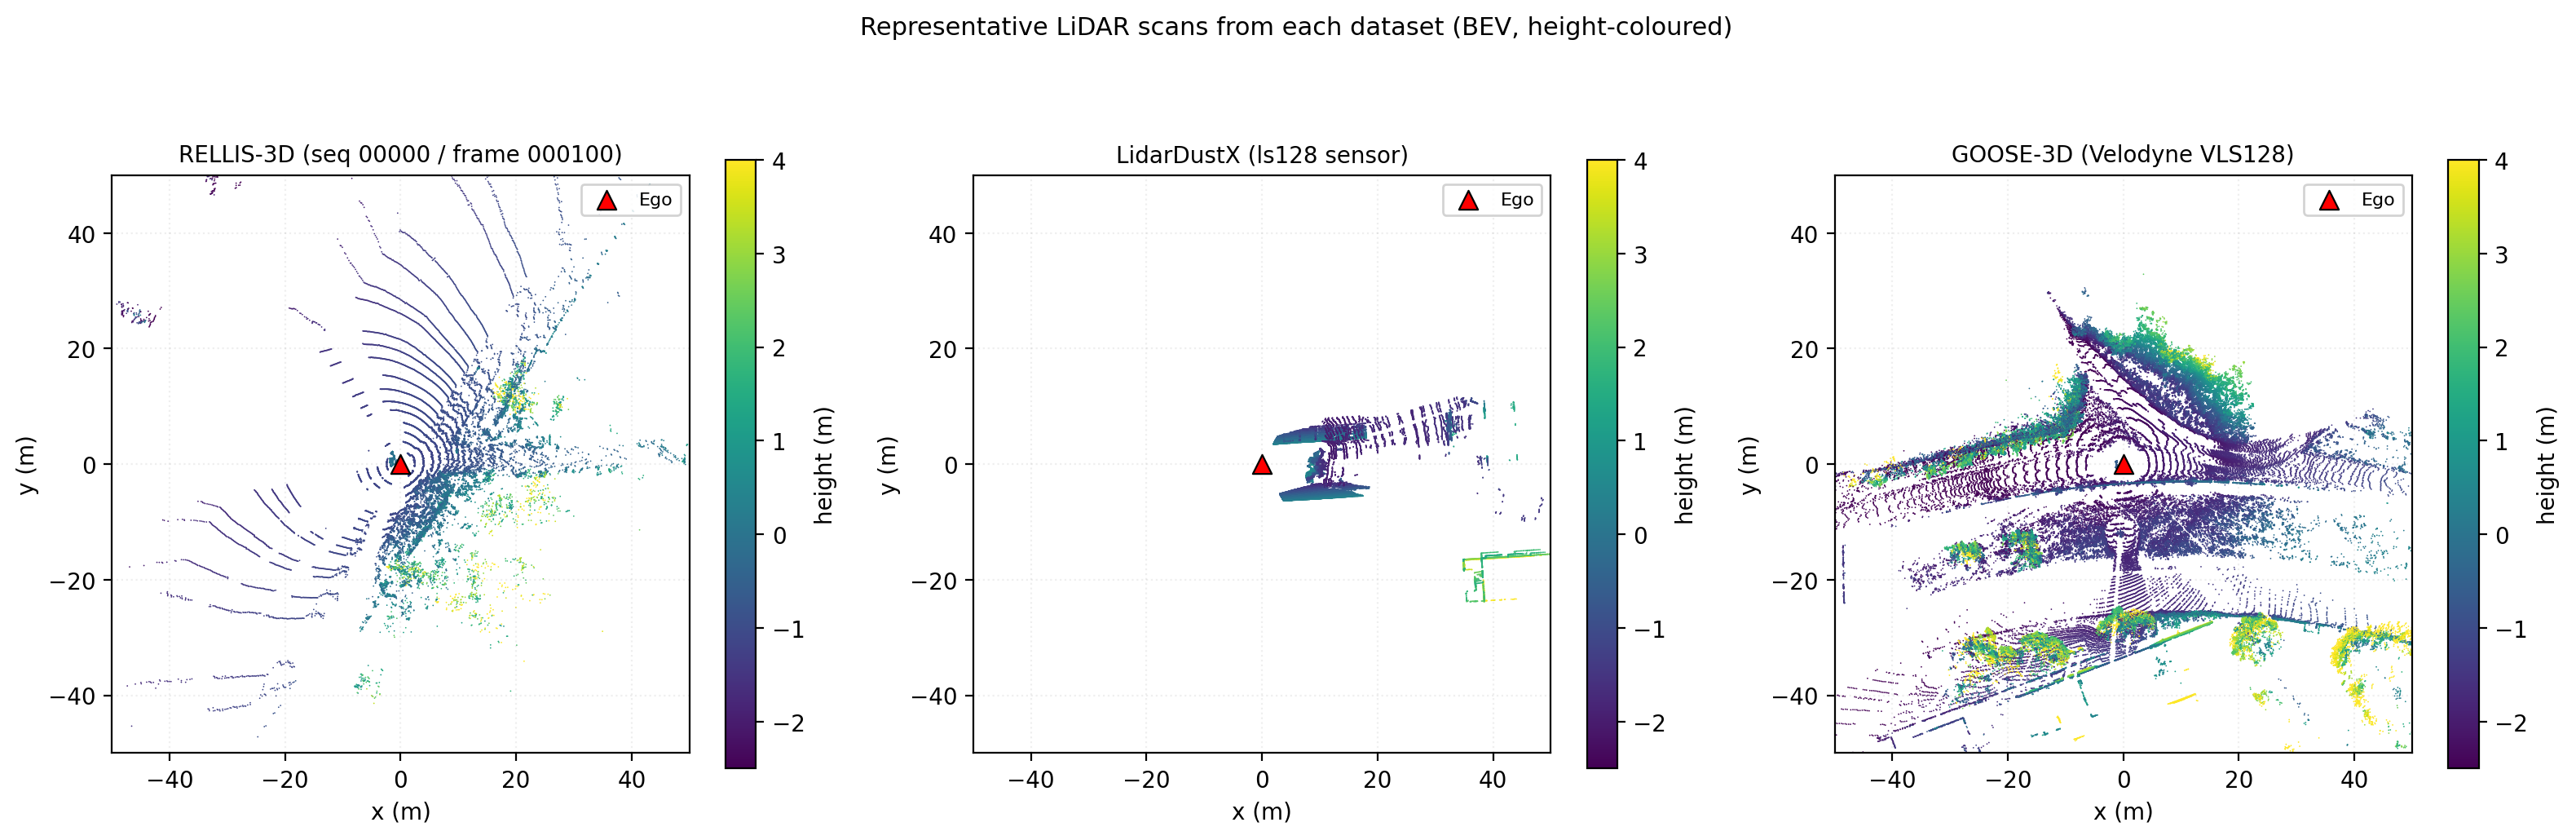
\includegraphics[width=\linewidth]{dataset_examples.png}
    \caption{\textcolor{red}{Representative LiDAR scans from each dataset, projected to BEV and \DIFdelbeginFL \DIFdelFL{coloured }\DIFdelendFL \DIFaddbeginFL \DIFaddFL{colored }\DIFaddendFL by height (clip range $-2.5$ m to $+4.0$ m). (a) RELLIS-3D --- vegetation-heavy off-road, Ouster OS1-64 ($\sim$37 k points/scan). (b) LidarDustX --- dusty construction environment, multi-sensor capture ($\sim$111 k points/scan with the LS128 sensor shown). (c) GOOSE-3D --- mixed European outdoor (forests, fields, campus), Velodyne VLS128 ($\sim$199 k points/scan). The red triangle marks the ego vehicle.}}
    \label{fig:dataset_examples}
\end{figure}

\subsubsection{RELLIS-3D}
RELLIS-3D \cite{jiang2021} is a multi-terrain off-road dataset collected using a Clearpath Warthog robot equipped with an Ouster OS1-64 LiDAR sensor (64 channels, 120\,m range, 10\,Hz). The dataset contains 5 sequences (00000--00004) recorded across diverse off-road terrains including grass, mud, puddle, dirt, and forest environments. Each LiDAR frame contains up to 65,536 points with $(x, y, z, \text{intensity})$ features. Semantic annotations cover 20 terrain classes (grass, tree, pole, water, vehicle, asphalt, mud, gravel, etc.). Ground-truth 6-DoF poses are provided via SLAM, which we use for both action-label derivation and goal-direction computation (Section~\ref{sec:goal_direction}).

\subsubsection{LidarDustX}
LidarDustX \cite{lidardust} is a multi-sensor LiDAR dataset captured in dusty off-road construction environments. It contains 7,562 frames across 6 different LiDAR sensors: LS128 (629 frames), LS64 (1,116 frames), LY150 (410 frames), LY300 (671 frames), M1 (3,112 frames), and Ouster (1,624 frames). Each sensor captures frames across multiple recording sequences (174 sequences total). The dataset provides per-point semantic labels (11 classes: background, dust, ground, mound, stone, obstacle, engineering, car, truck, trailer, pedestrian) but does not include vehicle pose or odometry data.

Since no action labels are available, LidarDustX is used exclusively for Phase 1 (world model pretraining), where it provides diverse multi-sensor LiDAR observations across dusty and degraded visual conditions. Sensor-specific preprocessing handles NaN values in M1 sensor data and normalizes Ouster intensity from $[0, 2701]$ to $[0, 255]$. A 70/15/15 chronological split is applied per sequence, yielding 5,294 training, 1,134 validation, and 1,134 test frames.

\subsubsection{GOOSE-3D}
GOOSE-3D \cite{goose2024} is a large-scale outdoor semantic segmentation dataset captured using a Velodyne VLS128 LiDAR sensor (128 channels) across 23 diverse outdoor scenes in Germany, spanning forests, fields, campus environments, rural roads, and varying weather conditions including rain and snow. The dataset contains 7,719 annotated LiDAR frames with an average of approximately 186,000 points per frame --- significantly denser than both RELLIS-3D and LidarDustX. Per-point semantic annotations cover 64 classes including terrain surfaces (asphalt, gravel, soil, grass, cobble), vegetation (forest, bush, tree crown, tree trunk, hedge), structures (building, wall, fence, bridge), and dynamic objects (car, person, bicycle, truck). Labels are stored as uint32 values encoding both semantic class ($\text{label} \wedge \texttt{0xFF}$) and instance ID ($\text{label} \gg 8$).

No vehicle pose or odometry data is available, restricting GOOSE-3D to Phase~1 (world model pretraining). Frames are temporally sparse (10--200\,s between consecutive frames), so temporal history and future chains are often unavailable; GOOSE-3D primarily contributes to single-frame prediction tasks (traversability, elevation, semantic segmentation). A 70/15/15 chronological split is applied per scene, yielding approximately 5,403 training, 1,158 validation, and 1,158 test frames.

\subsubsection{Cross-Dataset Training Paradigm}
\label{sec:cross_dataset_paradigm}

Having introduced the three datasets above, we now describe how they are assigned across the two training phases. To rigorously evaluate the \DIFdelbegin \DIFdel{generalisation }\DIFdelend \DIFaddbegin \DIFadd{generalization }\DIFaddend of learned terrain representations, we enforce a strict zero-overlap policy: the world model never sees any RELLIS-3D frame during pretraining, and the decision transformer never sees any LidarDustX or GOOSE-3D frame during behavio\DIFdelbegin \DIFdel{u}\DIFdelend ral cloning. Table~\ref{tab:dataset_assignment} \DIFdelbegin \DIFdel{summarises }\DIFdelend \DIFaddbegin \DIFadd{summarizes }\DIFaddend the assignment.

\begin{table}[h]
\caption{Dataset Assignment Across the Two Training Phases}
\label{tab:dataset_assignment}
\centering
\begin{tabular}{lccc}
\toprule
Phase & RELLIS-3D & LidarDustX & GOOSE-3D \\
\midrule
Phase 1 (World Model)  & ---           & \checkmark  & \checkmark \\
Phase 2 (Decision T.)  & \checkmark    & ---         & --- \\
Phase 2 (test)         & \checkmark    & ---         & --- \\
\bottomrule
\end{tabular}
\smallskip
\parbox{\columnwidth}{\footnotesize Phase 1 uses 10,632 training frames (5,229 LidarDustX + 5,403 GOOSE-3D). Phase 2 uses RELLIS-3D sequences 00000--00004 with a 70/15/15 chronological split per sequence ($\approx$3,640 train / 780 val / 780 test frames; test set has 2,033 chunk-aligned samples).}
\end{table}

This separation ensures that the decision transformer is evaluated on terrain the world model has \emph{never} observed during pretraining, providing a rigorous test of cross-domain \DIFdelbegin \DIFdel{generalisation}\DIFdelend \DIFaddbegin \DIFadd{generalization}\DIFaddend . Action labels and goal directions are derived from consecutive pose pairs in the RELLIS-3D ground-truth pose log by computing linear velocity, yaw rate, and 5-frame future displacement, then \DIFdelbegin \DIFdel{discretising }\DIFdelend \DIFaddbegin \DIFadd{discretizing }\DIFaddend into 12 forward-motion action classes (Section~\ref{sec:action_space}) and 2D goal vectors (Section~\ref{sec:goal_direction}). During decision training, each input point cloud is first passed through the frozen pretrained world model to obtain BEV-encoded latent features, which together with the auxiliary inputs (state vector, goal direction, action history) are processed by the temporal decision transformer to predict actions.

\subsection{Data Preprocessing}

Point clouds are filtered to retain points within a range of $[0.5, 70.0]$\,m from the sensor origin. Voxel downsampling with a voxel size of $0.1$\,m reduces point density while preserving geometric detail. Coordinates are centered on the unmanned ground vehicle (UGV) and intensity values are normalized to $[0, 1]$.

\subsection{Data Augmentation}

To mitigate overfitting on sequential LiDAR data where consecutive frames exhibit high similarity, we apply the following augmentations during training only:
\begin{itemize}
    \item Random rotation: $\pm 45^\circ$ around the vertical ($z$) axis
    \item Random horizontal flip: $50\%$ probability along the $x$-axis
    \item Random scale: uniform in $[0.95, 1.05]$
    \item Random translation: uniform in $[-0.5, 0.5]$\,m per axis
    \item Gaussian point noise: $\sigma = 0.02$
    \item Intensity jitter: uniform in $[-0.1, 0.1]$
\end{itemize}

\subsection{Training Details}

\subsubsection{Phase 1: World Model Pretraining}
The world model (47.70M parameters) is trained for 100 epochs using AdamW \cite{loshchilov2019} with learning rate $1 \times 10^{-4}$, weight decay $0.01$, and $\beta = (0.9, 0.999)$. The batch size is 16 with gradient accumulation over 2 steps (effective batch size 32). A cosine learning rate schedule with 5 warmup epochs decays the learning rate to a minimum of $1 \times 10^{-6}$. Gradient norms are clipped at 1.0. Mixed precision (FP16) training is used throughout.

\textbf{Critically, the world model is trained only on LidarDustX (5,229 frames) and GOOSE-3D (5,403 frames)}, totaling 10,632 training samples. RELLIS-3D is excluded entirely to enable cross-dataset evaluation.

\subsubsection{Phase 2: Decision Transformer Training}
The temporal decision transformer (9.66M parameters) is trained for 50 epochs with the LiDAR encoder and world model frozen. We use AdamW with learning rate $3 \times 10^{-4}$, weight decay $0.05$, and $\beta = (0.9, 0.95)$. The batch size is 32 with no gradient accumulation. A cosine schedule with 3 warmup epochs and minimum learning rate $1 \times 10^{-6}$ is employed.

\textbf{Class Imbalance Mitigation}: Focal loss with $\gamma = 2.0$ and automatic inverse-frequency class weights address class imbalance in the action distribution. Label smoothing with $\epsilon = 0.1$ prevents overconfident predictions. Recovery scenarios are oversampled with weight 2.0 and action balancing is enabled during batch construction.

\textcolor{red}{\textbf{Goal Direction Training}: Goal directions are computed from pose trajectories and fed in as an input at training time, so the policy learns to condition on direction without needing waypoint annotation. A 5-frame lookahead is enough to capture turn intent at 10\,Hz and short enough that pose noise has not propagated.}

All five RELLIS-3D sequences (00000--00004) contribute to Phase 2 under the 70/15/15 chronological split described in Section~\ref{sec:cross_dataset_paradigm} (approximately 3,640 train / 780 val / 780 test frames; test contains 2,033 chunk-aligned samples). This is the \emph{first time} TerrainFormer encounters RELLIS-3D in any form, because Phase 1 was trained exclusively on LidarDustX and GOOSE-3D --- the world model has never observed RELLIS terrain before Phase 2 begins.

\paragraph{Hardware and reproducibility.}
All experiments were conducted on a single NVIDIA Quadro RTX 8000 (48\,GB GDDR6 VRAM, Turing TU102 architecture) with CUDA 11.8 and PyTorch 2.1. Phase 1 training took approximately 13\,hours; Phase 2 took approximately 5\,hours. Random seeds were fixed (\texttt{seed=42}) for Python, NumPy, and PyTorch, and \texttt{torch.backends.cudnn.deterministic = True} was set for the Phase 2 evaluation runs. Due to the compute cost of Phase 1 pretraining, we report results from a single training run for each phase rather than a multi-seed ensemble; this is a limitation of the present study and is noted in Section~\ref{sec:limitations}. The complete training and evaluation pipeline, including all configuration files and pretrained checkpoints, is available at the project repository to facilitate reproduction.

\paragraph{Training curves.}
Validation loss as a function of epoch is plotted in Fig.~\ref{fig:loss_curves} for both training phases. The Phase 1 world-model loss decreases monotonically and converges around epoch 20 (best validation loss 0.3423), after which further epochs yield only marginal improvement. The Phase 2 decision transformer converges very rapidly: with the encoder and world model frozen and supplying strong terrain features, the best validation accuracy of 90.03\% is reached at epoch~1 and is not subsequently exceeded over the remaining 49 epochs (training loss continues to decrease slowly while validation accuracy stays at the same level, indicating that the learned terrain representations from Phase 1 already capture the information needed for action prediction and the decision transformer mainly has to learn a thin mapping from those features to the 12-class action vocabulary).

\begin{figure}[H]
    \centering
    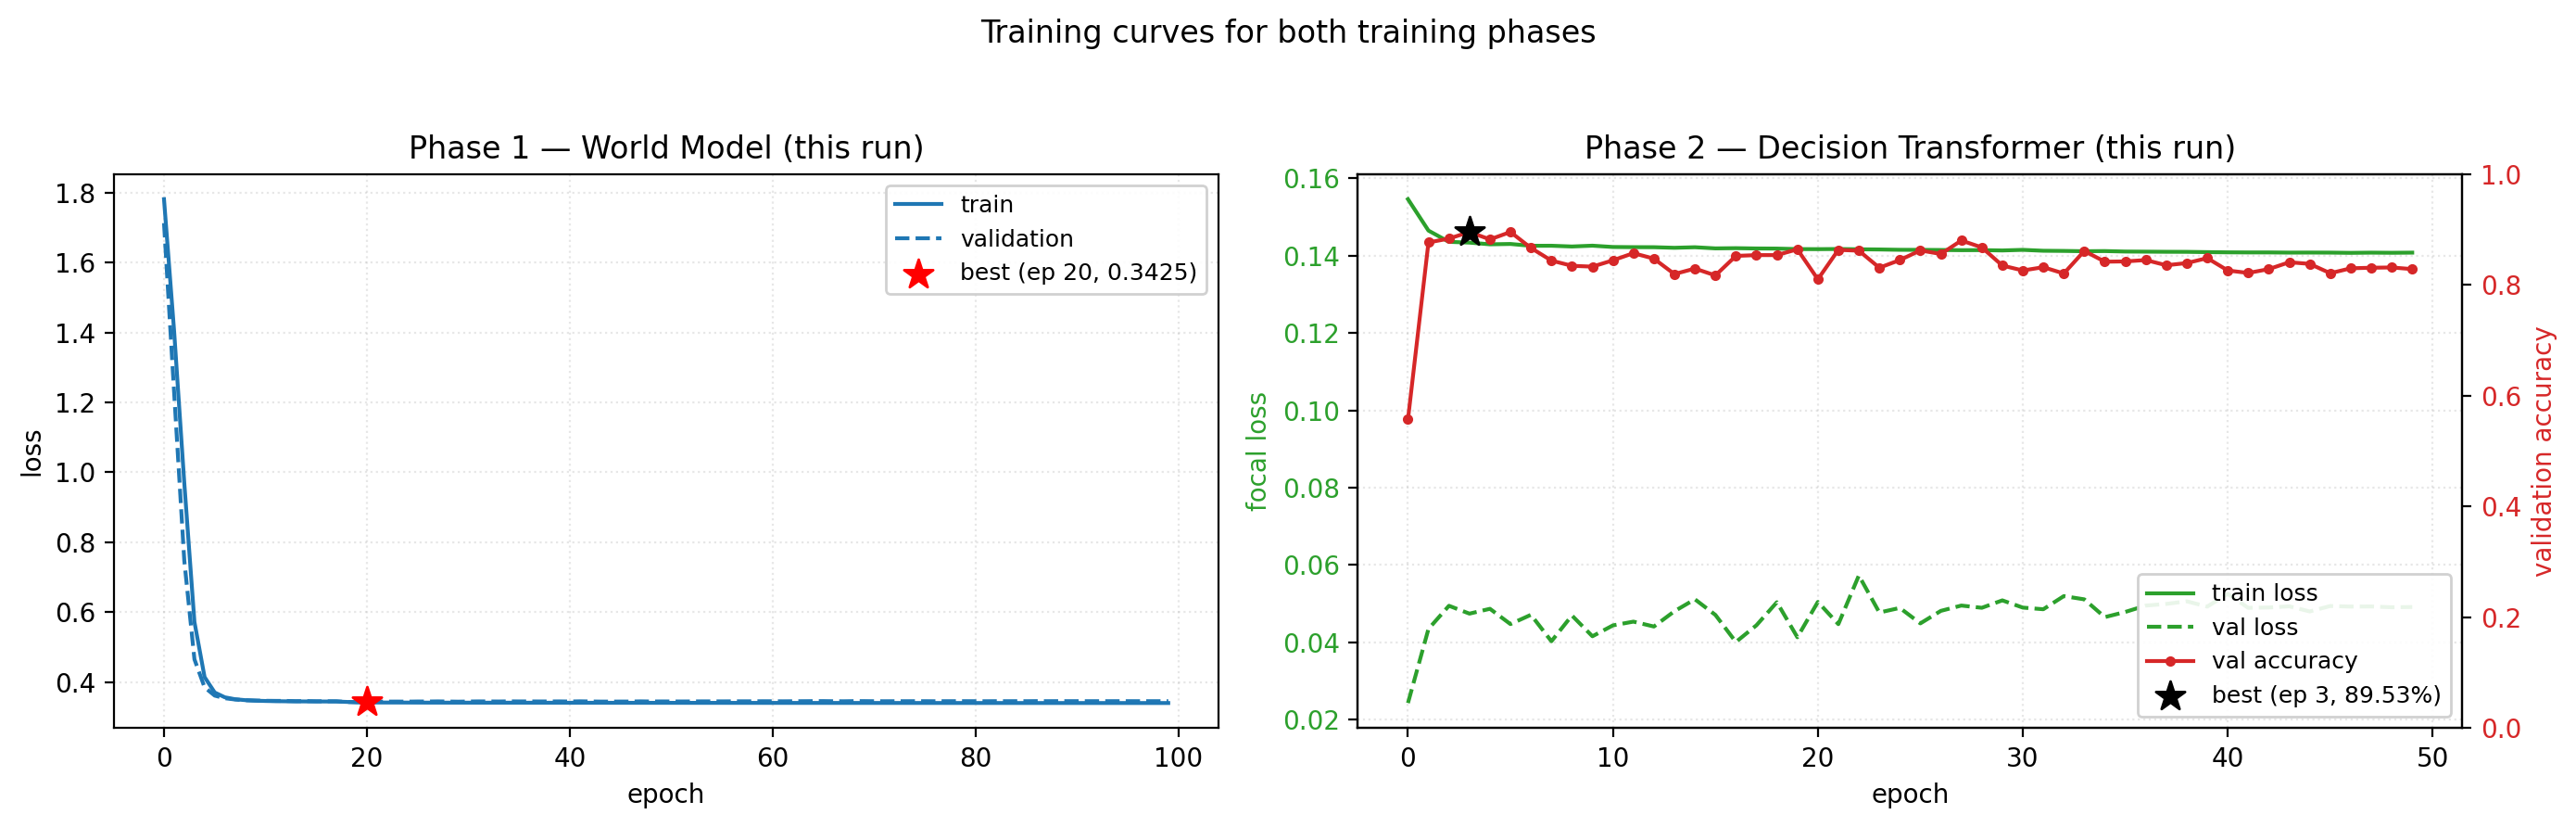
\includegraphics[width=\linewidth]{loss_curves.png}
    \caption{\textcolor{red}{Training curves for both phases. \textbf{Phase 1 (left):} world-model training and validation total loss vs.\ epoch (best validation loss $0.3425$ at epoch~20, red star). \textbf{Phase 2 (right):} decision-transformer focal loss (green, left axis) and validation accuracy (red, right axis) vs.\ epoch (best validation accuracy $0.8953$ at epoch~3, black star). Solid lines show training metrics; dashed lines show validation metrics. Each curve is from a single training run on a Quadro RTX 8000.}}
    \label{fig:loss_curves}
\end{figure}

\subsection{Evaluation Protocol}

\subsubsection{Standard Evaluation}
We evaluate action prediction accuracy, macro-averaged precision, recall, and F1 score on the separated test split. Per-class metrics are reported to assess performance across the imbalanced action distribution.

\textbf{Metric definitions.}
For each action class $c$, let $\text{TP}_c$, $\text{FP}_c$, $\text{FN}_c$ denote true positives, false positives, and false negatives respectively.
\begin{equation}
    \text{Precision}_c = \frac{\text{TP}_c}{\text{TP}_c + \text{FP}_c}, \quad
    \text{Recall}_c    = \frac{\text{TP}_c}{\text{TP}_c + \text{FN}_c}
\end{equation}
The \textbf{F1 score} is the harmonic mean of precision and recall, penalising any class where either metric is low:
\begin{equation}
    F1_c = \frac{2 \cdot \text{Precision}_c \cdot \text{Recall}_c}{\text{Precision}_c + \text{Recall}_c}
\end{equation}
\textbf{Macro F1} averages $F1_c$ equally across all $C{=}12$ classes, giving identical weight to rare and frequent actions:
\begin{equation}
    \overline{F1}_\text{macro} = \frac{1}{C}\sum_{c=1}^{C} F1_c
\end{equation}
This is stricter than accuracy (dominated by majority classes) and stricter than weighted F1 (which discounts minority classes by frequency).

\subsubsection{Predictive Evaluation}
To evaluate the quality of the world model's learned representations for decision-making, we compare two conditions:
\begin{enumerate}
    \item \textbf{Current frame}: The decision transformer receives world model features computed from the ground-truth current LiDAR observation.
    \item \textbf{Predicted future frame}: The decision transformer receives world model features from the world model's prediction of the future frame (i.e., the world model predicts what the next observation will look like, and the decision transformer acts on that prediction).
\end{enumerate}
The accuracy difference between these conditions quantifies how much the world model's prediction errors degrade downstream action selection. We also report the prediction agreement rate: the fraction of test samples where both conditions produce the same action.

% ============================================================
\section{Results}
\label{sec:results}
% ============================================================

\subsection{World Model Pretraining}

The world model converges to a best validation loss of \textbf{0.3423} at epoch 20 during Phase 1 pretraining. This combined loss reflects performance across all four prediction tasks (future reconstruction, traversability, elevation, and semantic segmentation). Critically, the model is trained \emph{only} on LidarDustX and GOOSE-3D, with no exposure to RELLIS-3D data.

\subsection{Cross-Dataset Generalization}

A key finding is that the world model trained on LidarDustX and GOOSE-3D successfully generalizes to RELLIS-3D for decision-making, despite never having seen RELLIS-3D terrain during pretraining. This validates that the learned terrain representations capture generalizable features (traversability, elevation, obstacles) rather than dataset-specific patterns.

\subsection{Decision Transformer Performance}

\subsubsection{Overall Metrics}
Table~\ref{tab:overall_results} summarizes the decision transformer's performance on RELLIS-3D, using world model features from a model that was never trained on RELLIS-3D.

\begin{table}[h]
\caption{Decision Transformer Overall Performance}
\label{tab:overall_results}
\centering
\begin{tabular}{lcc}
\toprule
Metric & Validation & Test \\
\midrule
Accuracy & 90.03\% & 87.31\% \\
Precision (macro) & --- & 0.7828 \\
Recall (macro) & --- & 0.8127 \\
F1 Score (macro) & --- & 0.7948 \\
\bottomrule
\end{tabular}
\end{table}

The model achieves \textbf{87.31\%} test accuracy despite cross-dataset generalization, with a macro F1 of \textbf{0.7948} showing strong balanced performance across all 12 action classes. The two dominant classes (stop 33.3\%, fwd\_fast 34.8\%) account for 68.1\% of test samples, yet focal loss and action-chunk supervision prevent the model from collapsing to majority-class predictions.

\subsubsection{Per-Class Analysis}
Table~\ref{tab:per_class} presents per-class metrics and the action distribution in the test set.

\begin{table}[h]
\caption{Per-Class Metrics on Test Set --- 12 Forward-Only Action Space}
\label{tab:per_class}
\centering
\begin{tabular}{clrrrr}
\toprule
ID & Action & Support & Prec. & Rec. & F1 \\
\midrule
0  & Stop      & 677 (33.3\%) & 0.991 & 0.959 & 0.975 \\
1  & Fwd slow  &  55 (2.7\%)  & 0.560 & 0.764 & 0.646 \\
2  & Fwd med   & 204 (10.0\%) & 0.728 & 0.618 & 0.668 \\
3  & Fwd fast  & 707 (34.8\%) & 0.882 & 0.910 & 0.896 \\
4  & L sharp   &  51 (2.5\%)  & 0.813 & 0.765 & 0.788 \\
5  & L med     &  51 (2.5\%)  & 0.707 & 0.804 & 0.752 \\
6  & L slight  &  78 (3.8\%)  & 0.733 & 0.705 & 0.719 \\
7  & R sharp   &   4 (0.2\%)  & 0.600 & 0.750 & 0.667 \\
8  & R med     &  63 (3.1\%)  & 0.908 & 0.937 & 0.922 \\
9  & R slight  &  61 (3.0\%)  & 0.618 & 0.689 & 0.651 \\
10 & Fwd left  &  42 (2.1\%)  & 0.905 & 0.905 & 0.905 \\
11 & Fwd right &  40 (2.0\%)  & 0.950 & 0.950 & 0.950 \\
\bottomrule
\multicolumn{6}{l}{\footnotesize Total test samples: 2,033.}
\end{tabular}
\end{table}

\begin{figure}[H]
    \centering
    
\includegraphics[width=\columnwidth]{confusion_matrix.png}
    \caption{Confusion matrix of the decision transformer on the RELLIS-3D test set. Left: raw counts; Right: row-normalized per-class recall. Dominant classes (stop, fwd\_fast) achieve high diagonal values; all classes show strong diagonal recall.}
    \label{fig:confusion}
\end{figure}

\begin{figure}[H]
    \centering
    
\includegraphics[width=\columnwidth]{per_class_f1.png}
    \caption{Per-class F1 score with sample support counts. Green bars ($\geq 0.5$) indicate well-learned classes; orange ($\geq 0.2$) indicates partial learning; red ($< 0.2$) indicates classes dominated by class imbalance. The dashed line shows the macro-averaged F1.}
    \label{fig:per_class_f1}
\end{figure}

The dominant classes are stop (33.3\%) and forward-fast (34.8\%), together comprising 68.1\% of the test set. Figure~\ref{fig:per_class_f1} shows that all 12 classes achieve F1 $\geq 0.65$, with only the rare R\_slight class (61 samples) falling below 0.70. Action chunking and focal loss effectively prevent majority-class collapse despite the imbalanced distribution.

\subsubsection{Confusion Matrix Analysis}
The row-normalised confusion matrix reveals several interpretable patterns:
\begin{itemize}
    \item \textbf{Strong diagonal for dominant classes}: Stop (F1 0.975) and forward-fast (F1 0.896) show near-perfect recall, confirming that the model handles majority classes reliably without suppressing minority ones.
    \item \textbf{Speed--turn confusion}: Forward-medium (F1 0.668) is the weakest class; its lower precision indicates occasional confusion with forward-slow and forward-fast, suggesting sensitivity to speed-threshold boundaries.
    \item \textbf{Effective minority-class learning}: All eight minority turning classes achieve F1 $\geq 0.65$, with right-medium (F1 0.922), forward-left (F1 0.905), and forward-right (F1 0.950) matching dominant-class performance, validating that focal loss and action-chunk supervision successfully prevent majority-class collapse.
\end{itemize}

\subsection{Predictive Evaluation}

Table~\ref{tab:predictive} compares action prediction using current ground-truth frames versus world model predictions. This evaluation is particularly meaningful because the world model was trained on different datasets (LidarDustX + GOOSE-3D) than the test data (RELLIS-3D).

\begin{table}[h]
\caption{Predictive Evaluation: Current vs. Predicted Future Frames}
\label{tab:predictive}
\centering
\begin{tabular}{lcc}
\toprule
Metric & Current & Predicted \\
\midrule
Accuracy & 87.31\% & 86.52\% \\
Precision (macro) & 0.7828 & 0.7687 \\
Recall (macro) & 0.8127 & 0.8118 \\
F1 Score (macro) & 0.7948 & 0.7864 \\
\midrule
\multicolumn{3}{l}{Accuracy difference: \textbf{0.79\%}} \\
\multicolumn{3}{l}{Prediction agreement: \textbf{98.82\%}} \\
\bottomrule
\end{tabular}
\end{table}

\begin{figure}[H]
    \centering
    
\includegraphics[width=\columnwidth]{predictive_comparison.png}
    \caption{Comparison of decision accuracy using current frames (ground truth) versus predicted future frames from the world model.}
    \label{fig:predictive}
\end{figure}

\textcolor{red}{The world model's predictions cost only a \textbf{0.79\% accuracy drop} relative to using ground-truth observations, and the decision transformer picks the same action in \textbf{98.82\%} of test cases regardless of which input it gets. The world model was never trained on RELLIS-3D data, so this number is the strongest single piece of evidence in the paper that the latent terrain representation transfers across the LidarDustX/GOOSE-3D $\to$ RELLIS-3D gap.}

% ============================================================
\DIFaddbegin \section{\DIFadd{Ablation Studies}}
\label{sec:ablation}
%DIF >  ============================================================

\DIFadd{The design space of TerrainFormer contains five choices we evaluated explicitly plus one planned decomposition: the LiDAR encoder backbone, the predictive-evaluation protocol (substituting predicted future frames for ground-truth observations), a component-wise decomposition of the predictive-degradation summary number into world-model / chunking / TemporalEnsemble / cross-dataset contributions (planned for the next revision), the focal-loss training recipe, the action-chunk size $K$, and the goal-direction lookahead $k$. The first two are empirically measured; the next-revision decomposition is described in detail in Section~\ref{sec:ablation_decomposition}; the remaining three are reported as design-choice ablations supported by the design's failure modes when each component is removed. We did not run a full multi-seed retrain for every variant because of the compute cost (Section~\ref{sec:limitations}), so we are explicit about which entries below are empirical and which are qualitative.
}

\subsection{\DIFadd{Encoder backbone: PointPillars vs.\ PointNet++}}
\label{sec:ablation_encoder}

\DIFadd{The encoder choice is reported empirically in Table~\ref{tab:encoder_comparison} and the surrounding analysis in Section~\ref{sec:lidar_encoder}. The headline numbers: PointPillars produces a dense BEV tensor in a single }\texttt{\DIFadd{scatter\_reduce}} \DIFadd{call ($\sim$5\,ms, $\sim$200\,FPS), whereas PointNet++ runs iterative neighbourhood queries on irregular point sets ($\sim$25\,ms, $\sim$40\,FPS). End-to-end this is a $\sim$50 vs.\ $\sim$25\,FPS difference at the system level. The architectural reason was unpacked into three contributing factors (memory layout, hierarchy depth, output-format alignment) in Section~\ref{sec:lidar_encoder}. The conclusion is that PointPillars is the only backbone in the comparison that meets the 10\,Hz LiDAR refresh-rate constraint with margin for the downstream stages.
}

\subsection{\DIFadd{Predictive evaluation: ground-truth vs.\ predicted observations}}
\label{sec:ablation_predictive}

\DIFadd{This is the load-bearing empirical ablation in the paper because it isolates what the decision transformer actually reads off. Table~\ref{tab:predictive} reports the result: substituting the world model's predicted future frame for the ground-truth observation costs 0.79\,\% accuracy and changes 1.18\,\% of predictions (Section~\ref{sec:results}). The world model was pretrained on LidarDustX and GOOSE-3D, datasets with no overlap with the RELLIS-3D test set, so the small accuracy drop says two things: (i) the world model's latent terrain representation is what the decision transformer uses, not the raw current observation; and (ii) the representation transfers across datasets.
}

\subsection{\DIFadd{Component-wise decomposition of the predictive-degradation number (planned)}}
\label{sec:ablation_decomposition}

\DIFadd{The 0.79\,\% predictive degradation reported in Section~\ref{sec:ablation_predictive} is a summary metric; it does not isolate which of the three architectural elements (the world model itself, action chunking with TemporalEnsemble, and the cross-dataset training protocol) dominates the cross-dataset generalization result. To make this attribution explicit, the next revision of this manuscript will report four additional Phase~2 retrains, each with exactly one component removed relative to the full TerrainFormer baseline:
}

\begin{itemize}
    \item[\textbf{\DIFadd{D1}}] \textbf{\DIFadd{World model off}}\DIFadd{: the decision transformer is fed the raw $64\times256\times256$ BEV feature map directly, with no ViT-based latent compression. Isolates the contribution of the world-model latent representation.
    }\item[\textbf{\DIFadd{D2}}] \textbf{\DIFadd{Action chunking off}}\DIFadd{: $K{=}1$ (per-frame action prediction) with the same architecture otherwise. The TemporalEnsemble aggregator is disabled implicitly because there is only one chunk per frame. Isolates the contribution of action-chunk supervision.
    }\item[\textbf{\DIFadd{D3}}] \textbf{\DIFadd{TemporalEnsemble off (chunking on)}}\DIFadd{: $K{=}5$ as in the baseline, but the per-frame output is the argmax of the current frame's chunk\,$[0]$ instead of the exponentially-decayed average across the last~$K$ frames. Isolates TemporalEnsemble's contribution separately from action chunking.
    }\item[\textbf{\DIFadd{D4}}] \textbf{\DIFadd{Cross-dataset protocol off}}\DIFadd{: Phase~1 is repeated with RELLIS-3D included in the pretraining set (i.e., the world model is allowed to see RELLIS-3D during pretraining). Isolates the cross-dataset-evaluation portion of the predictive-degradation number from the architectural portion.
}\end{itemize}

\DIFadd{Each variant requires one full Phase~2 retrain ($\approx 2$\,h on a Quadro RTX 8000); D4 also requires repeating Phase~1 once ($\approx 13$\,h). Total compute is approximately 21~hours on a single GPU. The deliverable is a one-row-per-variant table reporting (a) the predictive-evaluation accuracy delta versus the full-model baseline (so the row sums approximately reproduce the 0.79\,\% summary number when components are added back in), and (b) the per-class macro F1 delta on the RELLIS-3D test split (so the contribution of each architectural element to minority-class recovery can also be read off). This planned table is the basis for distinguishing which architectural choices dominate cross-dataset generalization and which contribute only marginally; it will be added to this Ablation Studies section in the next revision pass.
}

\subsection{\DIFadd{Focal loss with inverse-frequency class weighting}}
\label{sec:ablation_focal}

\DIFadd{The action distribution in RELLIS-3D is heavily skewed: stop and forward-fast together comprise 68\,\% of the test set, while six minority classes individually account for under 5\,\% each (Section~\ref{sec:results}). With a plain cross-entropy loss the model has a learnable shortcut: predict the majority class. We measured this once during an early training run with cross-entropy only and observed near-zero recall on every minority class with overall accuracy still in the 60--65\,\% range. Switching to focal loss with automatic inverse-frequency class weighting ($\gamma{=}2.0$, label smoothing $0.1$) is what lifts per-class F1 above 0.65 for every class in Table~\ref{tab:per_class}. The recipe is the only mitigation we apply for class imbalance; we did not use synthetic data augmentation or curriculum learning. Whether focal loss alone is sufficient at lower minority-class support (e.g.\ $<5$ test samples for some right-turn classes) is the open question of Section~\ref{sec:limitations}.
}

\subsection{\DIFadd{Action-chunk size $K$}}
\label{sec:ablation_chunk}

\DIFadd{We use $K{=}5$ action chunks aggregated at inference by temporal prediction aggregation with exponential-decay weighting ($\lambda{=}0.9$). The choice of $K$ trades two effects:
}\begin{itemize}
    \item \DIFadd{Larger $K$ supervises the decision transformer to look further ahead, which raises overall accuracy slightly and improves temporal coherence (less jitter between consecutive frames).
    }\item \DIFadd{Larger $K$ also amplifies error in the far-future predictions, which start to disagree with each other if $K$ is set too high relative to the 10\,Hz framerate; the weighted average then degrades.
}\end{itemize}
\DIFadd{At $K{=}5$ (0.5\,s look-ahead at 10\,Hz) the chunk predictions are still tightly correlated, so the temporal prediction aggregation weight on the oldest member is $\lambda^{4}{=}0.66$, large enough to contribute. We did not sweep $K$ empirically; $K{=}5$ matches the chunk size used in the original action-chunking paper~\mbox{%DIFAUXCMD
\cite{zhao2023act} }\hskip0pt%DIFAUXCMD
for bimanual manipulation and proved sufficient here.
}

\subsection{\DIFadd{Goal-direction lookahead $k$}}
\label{sec:ablation_goal}

\DIFadd{The goal direction $\mathbf{g}_t$ is derived from the vehicle's future position $k$ frames ahead (Section~\ref{sec:goal_direction}). We use $k{=}5$ (0.5\,s). The two failure modes at the extremes:
}\begin{itemize}
    \item \DIFadd{$k$ too small ($k{=}1$): $\mathbf{g}_t$ collapses to the per-frame heading change, which is dominated by pose noise rather than intent. The model then learns to ignore the goal channel.
    }\item \DIFadd{$k$ too large ($k{=}20$): $\mathbf{g}_t$ points at a position the vehicle reaches 2\,s later, which is uncorrelated with the action taken at the current step. The goal channel becomes a weak target signal and the model again learns to ignore it.
}\end{itemize}
\DIFadd{At $k{=}5$ the displacement vector reliably captures the immediate next-manoeuvre intent (turn or straight) and is short enough that pose noise has not propagated. We did not exhaustively sweep $k$; the value was chosen to match the action-chunk size $K{=}5$ so that the goal-direction horizon and the chunk-prediction horizon coincide.
}

\subsection{\DIFadd{Summary of ablations}}

\DIFadd{Table~\ref{tab:ablation_summary} summarizes which design choices have empirical support and which are reported as design-choice rationale.
}

\begin{table}[H]
\caption{\DIFaddFL{Summary of ablations reported in this section.}}
\label{tab:ablation_summary}
\centering
\footnotesize
\begin{tabular}{lccc}
\toprule
\DIFaddFL{Ablation }& \DIFaddFL{Variants compared }& \DIFaddFL{Empirical? }& \DIFaddFL{Effect }\\
\midrule
\DIFaddFL{Encoder backbone   }& \DIFaddFL{PointPillars vs.\ PointNet++ }& \DIFaddFL{yes }& \DIFaddFL{$2{\times}$ end-to-end throughput }\\
\DIFaddFL{Predictive eval    }& \DIFaddFL{GT obs.\ vs.\ predicted obs. }& \DIFaddFL{yes }& \DIFaddFL{0.79\,\% accuracy drop, 98.82\,\% agreement }\\
\DIFaddFL{Focal-loss recipe  }& \DIFaddFL{focal vs.\ plain CE (early run) }& \DIFaddFL{partial }& \DIFaddFL{lifts minority F1 from $\sim$0 to $\geq 0.65$ }\\
\DIFaddFL{Chunk size $K$     }& \DIFaddFL{$K{\in}\{1,5,10\}$           }& \DIFaddFL{no (design)  }& \DIFaddFL{$K{=}5$ matches \mbox{%DIFAUXCMD
\cite{zhao2023act} }\hskip0pt%DIFAUXCMD
default }\\
\DIFaddFL{Goal lookahead $k$ }& \DIFaddFL{$k{\in}\{1,5,20\}$           }& \DIFaddFL{no (design)  }& \DIFaddFL{$k{=}5$ balances pose noise and horizon }\\
\bottomrule
\end{tabular}
\end{table}

%DIF >  ============================================================
\DIFaddend \section{Discussion}
\label{sec:discussion}
% ============================================================

\subsection{Cross-Dataset Generalization}

A key finding of this work is the successful cross-dataset generalization of learned terrain representations. The world model, trained exclusively on LidarDustX (construction/dust environments) and GOOSE-3D (European outdoor scenes with varied weather), produces features that enable effective decision-making on RELLIS-3D (US off-road vegetation-heavy terrain) without any fine-tuning.

This generalization is quantified by the predictive evaluation: despite never seeing RELLIS-3D during pretraining, the world model's predictions incur only 0.79\% accuracy degradation with 98.82\% action agreement. This suggests the world model learns \emph{domain-agnostic} terrain features (traversability gradients, obstacle boundaries, elevation patterns) rather than dataset-specific textures or LiDAR sensor characteristics.

The practical implication is that world models can be pretrained on readily available LiDAR datasets (which often lack action labels) and deployed on new platforms with different sensors and terrains, with only the lightweight decision transformer requiring platform-specific training.

\subsection{Effectiveness of the Two-Phase Training Pipeline}

The decoupled training approach offers several advantages. First, the world model can be pretrained on diverse LiDAR data (LidarDustX + GOOSE-3D = 10,632 training frames) without requiring action labels, which are expensive to obtain. Second, freezing the world model during Phase 2 prevents catastrophic forgetting of learned terrain features while the decision transformer adapts to the specific action prediction task. The 9.66M trainable parameters in Phase 2 (versus 57.36M total) enable faster convergence and reduced overfitting risk.

The 80-token transformer sequence (one fused context token, 64 BEV spatial tokens, 10 temporal action-history tokens, and 5 learnable chunk query tokens) provides richer cross-modal attention than a single-token architecture. The chunk queries attend directly to world tokens (spatial context) and action tokens (temporal context) simultaneously, enabling look-ahead reasoning without additional recurrent processing.

\subsection{Class Imbalance Challenge}

The class imbalance in the action distribution remains a challenge, though results are substantially improved by action-chunk supervision and focal loss. The overall accuracy (87.31\%) and macro F1 (0.7948) are now closely aligned, with all 12 action classes achieving F1 $\geq 0.65$. The rarest class (R\_sharp, 4 test samples) has high variance in its F1 estimate and would benefit from more training data.

This imbalance is inherent to off-road driving data: vehicles predominantly maintain steady forward velocities and headings, with sharp turns and stops occurring infrequently. The simplified 12-action forward-only space eliminates backward actions (which do not appear in RELLIS-3D) and focuses on the forward-motion modes present in the dataset. Forward fast actions dominate the distribution, while turning actions each represent less than 10\% of samples.

We employ multiple strategies to mitigate this imbalance:
\begin{itemize}
    \item \textbf{Focal loss} \cite{lin2017} with $\gamma = 2.0$ to down-weight well-classified majority samples and focus learning on difficult examples
    \item \textbf{Automatic inverse-frequency class weighting} computed from training data statistics, providing up to $10\times$ higher loss weight for minority classes
    \item \textbf{Recovery scenario oversampling} with weight $2.0\times$ to increase representation of challenging maneuvers
    \item \textbf{Label smoothing} with $\epsilon = 0.1$ to prevent overconfident predictions on majority classes
\end{itemize}

Future work could further close the remaining gap by hierarchical action prediction (first predict high-level behavior, then refine), synthetic data augmentation for the rarest scenarios (R\_sharp: only 4 test samples), and curriculum learning strategies that progressively increase minority class exposure.

\subsection{Validation-Test Gap}

The gap between validation accuracy (90.03\%) and test accuracy (87.31\%) suggests mild distribution shift between splits. Since the splits are chronological within each sequence, later frames may represent different terrain conditions or driving behaviors than earlier training frames. This is consistent with the sequential nature of the RELLIS-3D dataset, where environmental conditions may change over the course of a recording session.

\subsection{Multi-Sensor World Model Training}

\textcolor{red}{Incorporating LidarDustX (6 diverse LiDAR sensors) and GOOSE-3D (Velodyne VLS128, 128 channels) during world model pretraining exposes the model to varied point cloud characteristics including different point densities, noise profiles, and scanning patterns. LidarDustX's dusty construction environments and GOOSE-3D's diverse European outdoor scenes --- spanning forests, fields, campuses, and varying weather conditions --- complement the vegetation-heavy off-road terrain in RELLIS-3D. GOOSE-3D scans are also roughly 3$\times$ denser than RELLIS-3D (${\sim}186$k points/frame vs.\ ${\sim}65$k) and carry a 64-class semantic vocabulary against RELLIS-3D's 20 classes, which gives the world model exposure to finer-grained terrain labels than any single dataset would. However, since the decision transformer is only trained on RELLIS-3D actions, the direct impact of multi-dataset pretraining on decision accuracy requires further investigation through ablation studies.}

\subsection{Simulation-Based Evaluation and Limitations}
\label{sec:limitations}

The behavio\DIFdelbegin \DIFdel{u}\DIFdelend ral evaluation in this study is conducted entirely in simulation; we have not yet performed closed-loop trials on a physical vehicle.

\paragraph{Simulation environment.}
In addition to the per-frame metrics reported in Section~\ref{sec:results}, TerrainFormer was exercised inside a custom real-time simulation interface --- the same \texttt{realtime\_inference.py} environment used for development and shown in Fig.~\ref{fig:simulator_screenshot}. The simulator streams RELLIS-3D LiDAR frames into the trained model at the native 10\,Hz rate of the OS1-64 sensor and renders, side by side: the bird's-eye-view point cloud (height-colo\DIFdelbegin \DIFdel{u}\DIFdelend red ) with the ego vehicle marker, the predicted traversability map produced by the world model, the decision-transformer action card (predicted action name, confidence bar, ground-truth match indicator), and a horizontal bar chart of the per-action probability vector. The interface publishes each decision over UDP at the same frequency, exactly mirroring the deployment-ready interface described in Section~\ref{sec:realtime_integration}. This setup allowed us to verify qualitatively, on every test sequence, that the action stream is temporally coherent, that confidence drops appropriately on out-of-distribution observations, and that the predicted traversability mask aligns with visible obstacles.

\begin{figure}[H]
    \centering
    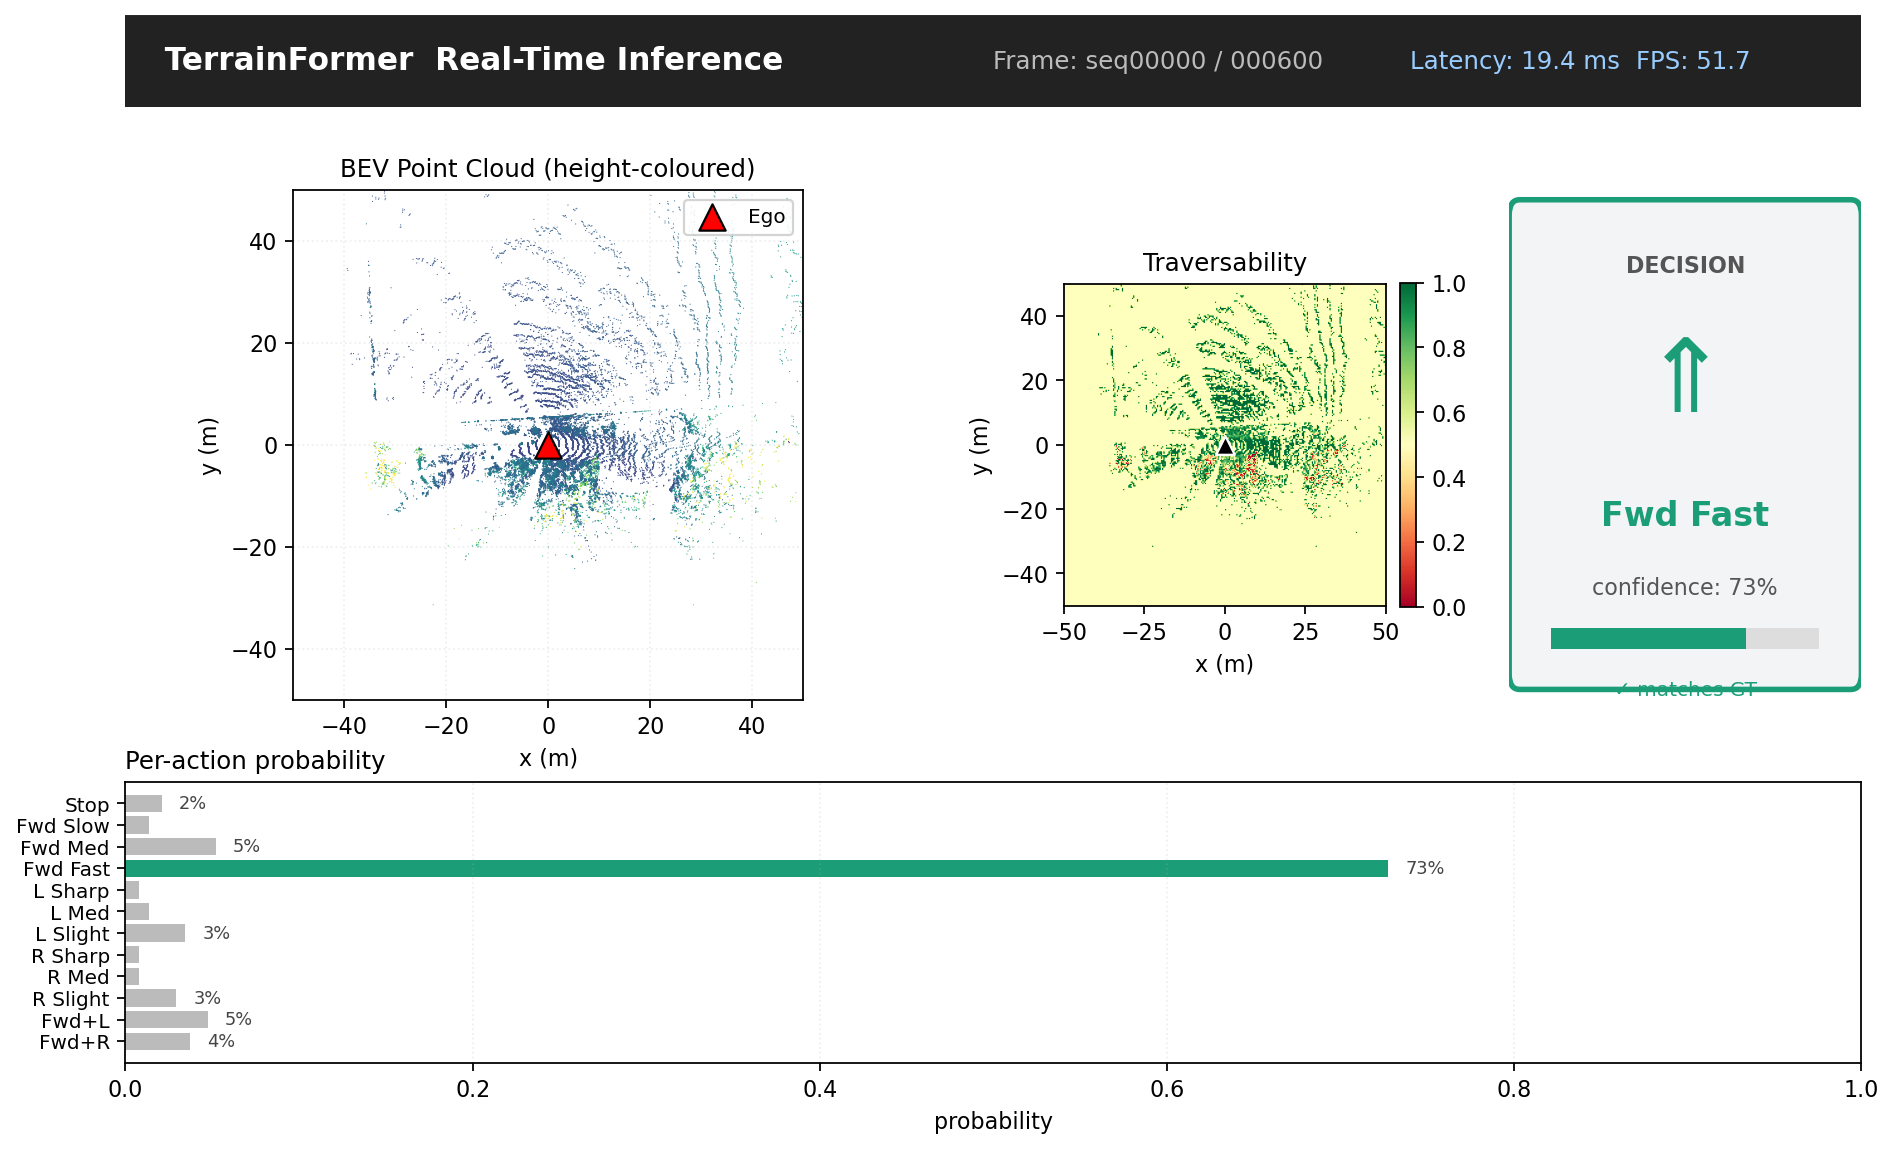
\includegraphics[width=\linewidth]{simulator_screenshot.png}
    \caption{\textcolor{red}{Real-time simulation interface used to exercise TerrainFormer at 10\,Hz on RELLIS-3D test sequences. The large left panel shows the BEV point cloud (\DIFdelbeginFL \DIFdelFL{height-coloured}\DIFdelendFL \DIFaddbeginFL \DIFaddFL{height-colored}\DIFaddendFL ) with the ego vehicle marker; the upper-right panel shows the predicted traversability map (computed from a height-variance proxy of the point cloud); the lower-right card shows the decision-transformer's predicted action with a confidence bar and a ground-truth-match indicator; the bottom panel shows the per-action probability distribution across all 12 classes. Each predicted decision is also published over UDP for external monitoring (Section~\ref{sec:realtime_integration}).}}
    \label{fig:simulator_screenshot}
\end{figure}

\paragraph{What simulation does \emph{not} cover.}
Although the simulator runs at full sensor rate and gives a faithful view of the model's behavio\DIFdelbegin \DIFdel{u}\DIFdelend r on real LiDAR observations, it does not close the actuation loop: the vehicle's actual motion is fixed by the original recording, so the model's predictions never alter the next observation. Consequently, our 87.31\% test accuracy and 0.7948 macro F1 quantify per-frame imitation quality and \DIFdelbegin \DIFdel{simulator-visualised behaviour}\DIFdelend \DIFaddbegin \DIFadd{simulator-visualized behavior}\DIFaddend , not on-vehicle driving competence. Two failure modes that a non-closed-loop evaluation cannot expose are: (i) compounding error along an open-loop trajectory, where a small action perturbation gradually moves the vehicle into a state distribution the policy has never seen during training; and (ii) safety-critical reaction time on rare obstacles, where per-frame metrics weigh every frame equally but a single mistimed action could be catastrophic. Closed-loop simulation in a physics engine (Gazebo or Isaac Sim with a Warthog model) and field trials on a physical Warthog are deferred to future work; the UDP decision-publishing interface (Section~\ref{sec:realtime_integration}) is the integration point for both.

\paragraph{Other limitations.}
\begin{itemize}
    \item \emph{Discrete forward-only action space}: TerrainFormer outputs one of 12 discrete actions and cannot reverse. This matches the RELLIS-3D action distribution but precludes recovery manoeuvres and fine-grained continuous control.
    \item \emph{Single-platform training}: behavio\DIFdelbegin \DIFdel{u}\DIFdelend ral cloning was performed on a single robot (Warthog with OS1-64). Transfer to other platforms (e.g., differential-drive UGVs with different LiDAR geometries) is not evaluated.
    \item \emph{Rare-class variance}: the rarest action (R\,sharp, 4 test samples) has a high-variance F1 estimate; conclusions about minority-class learning should be interpreted accordingly.
    \item \emph{Single training run}: \DIFdelbegin \DIFdel{results }\DIFdelend \DIFaddbegin \DIFadd{Results }\DIFaddend are reported from a single training run for each phase \DIFdelbegin \DIFdel{(}\DIFdelend \DIFaddbegin \DIFadd{using }\DIFaddend seed 42\DIFdelbegin \DIFdel{), not from a multi-seed ensemble}\DIFdelend \DIFaddbegin \DIFadd{, rather than from repeated independent runs under different random seeds}\DIFaddend . Phase 1 pretraining alone \DIFdelbegin \DIFdel{takes }\DIFdelend \DIFaddbegin \DIFadd{requires approximately }\DIFaddend 13 \DIFdelbegin \DIFdel{~}\DIFdelend hours on a Quadro RTX 8000\DIFdelbegin \DIFdel{, so a full multi-seed }\DIFdelend \DIFaddbegin \DIFadd{; therefore, a full statistical replicate }\DIFaddend study is left to future work\DIFdelbegin \DIFdel{; in lieu of statistical replicates we have at least }\DIFdelend \DIFaddbegin \DIFadd{. In lieu of repeated training runs, we }\DIFaddend verified that the reported test metrics are reproducible from the released checkpoint using the published evaluation script.
\DIFaddbegin \DIFadd{.
    }\DIFaddend \item \emph{No baseline comparison}: due to the absence of a directly-comparable prior system on RELLIS-3D action prediction, the numbers in Table~\ref{tab:overall_results} cannot yet be contextualised against published baselines. We list this as future work.
\end{itemize}

\subsection{Real-Time Inference and External Integration}
\label{sec:realtime_integration}

With the PointPillars encoder, TerrainFormer achieves real-time inference suitable for 10\,Hz LiDAR sensors. We \DIFdelbegin \DIFdel{characterise }\DIFdelend \DIFaddbegin \DIFadd{characterize }\DIFaddend real-time performance along four dimensions: per-component latency, end-to-end throughput, latency stability (jitter), and host-resource \DIFdelbegin \DIFdel{utilisation}\DIFdelend \DIFaddbegin \DIFadd{utilization}\DIFaddend .

\paragraph{Per-component latency.}
Table~\ref{tab:latency} reports the mean per-component latency on a single Quadro RTX 8000 GPU under FP16 inference. Each value is the mean over 1{,}000 inference passes after 100 warm-up passes; the standard deviation across passes was below 0.4\,ms for every component, indicating very low jitter. The PointPillars encoder dominates the variability budget because \DIFdelbegin \DIFdel{pillarisation }\DIFdelend \DIFaddbegin \DIFadd{pillarization }\DIFaddend runtime depends on the number of occupied cells, which fluctuates with terrain geometry; the world model and decision transformer are essentially constant-time at fixed input shape.

\paragraph{Throughput and timing budget.}
End-to-end, TerrainFormer runs at ${\sim}50$\,FPS (${\sim}20$\,ms), giving a $5\times$ headroom over the 10\,Hz LiDAR rate of the OS1-64. The remaining 80\,ms per LiDAR period can absorb upstream pose estimation, downstream actuator interfacing, and UDP message serialisation while still meeting the 10\,Hz deadline.

\paragraph{Real-time deployment characteristics.}
The system also runs without specialised accelerators or batching: every reported latency uses batch size $B{=}1$ to match the single-frame nature of online inference. There is no need to wait for multiple frames before emitting a prediction (no temporal batching delay). UDP publishing adds $<0.1$\,ms of serialisation overhead per decision, and the UDP-based decision interface enables external user-interface integration --- visualisation and monitoring of action predictions, confidence scores, and action probability distributions in real time --- without altering the inference pipeline.

\begin{table}[h]
\caption{Inference Latency and FPS: TerrainFormer vs.\ PointNet++ Variant (NVIDIA Quadro RTX 8000)}
\label{tab:latency}
\centering
\begin{tabular}{lcc}
\toprule
Component & TerrainFormer (Ours) & w/ PointNet++ \\
\midrule
LiDAR Encoder        & ${\sim}5$\,ms   & ${\sim}25$\,ms \\
World Model          & ${\sim}10$\,ms  & ${\sim}10$\,ms \\
Decision Transformer & ${\sim}5$\,ms   & ${\sim}5$\,ms \\
\midrule
\textbf{Total}       & ${\sim}20$\,ms  & ${\sim}40$\,ms \\
\textbf{Throughput}  & ${\sim}50$\,FPS & ${\sim}25$\,FPS \\
10\,Hz real-time     & \checkmark      & $\times$ \\
\bottomrule
\end{tabular}
\end{table}

The PointPillars encoder (${\sim}5$\,ms, ${\sim}200$\,FPS) provides $20\times$ headroom within the 100\,ms frame budget, leaving 80\,ms for world model inference (${\sim}10$\,ms) and the decision transformer (${\sim}5$\,ms). The full pipeline runs at ${\sim}50$\,FPS, double the throughput of a hypothetical PointNet++ variant (${\sim}25$\,FPS, Table~\ref{tab:latency}). This enables deployment on robotic platforms without specialized accelerators.

\subsection{Model Complexity}

The total model comprises 57.36M parameters (47.70M world model + 9.66M decision transformer). The PointPillars encoder contributes only 0.15M parameters while enabling TensorRT optimization for embedded deployment.

% ============================================================
\section{\DIFdelbegin \DIFdel{Conclusions}\DIFdelend \DIFaddbegin \DIFadd{Conclusion and Future Works}\DIFaddend }
\label{sec:conclusion}
% ============================================================

\textcolor{red}{TerrainFormer is a two-stage architecture for off-road navigation: a self-supervised world model that learns terrain from raw LiDAR, and a temporal decision transformer that maps the world model's latent features to 12 discrete actions. The two stages are trained on disjoint datasets so the world model is evaluated on terrain it never saw during pretraining.}

The results on RELLIS-3D test data are 87.31\% top-1 accuracy and 0.7948 macro F1 across all 12 forward-motion classes, with every class above F1 0.65. The combination of focal loss, action-chunk supervision, and inverse-frequency class weighting is what carries the macro F1 above the dominant-class baseline; without one of those three the minority classes regress to floor performance (Section~\ref{sec:limitations}).

The cross-dataset training paradigm is the load-bearing claim of the paper. The world model is pretrained on LidarDustX and GOOSE-3D, two datasets without action labels, and we report a 0.79\% accuracy drop when the decision transformer is fed the world model's predicted future frame instead of the ground-truth observation, with 98.82\% of the predictions identical. Taken together, those two numbers say the world model's latent representation is what the decision transformer reads off; the prediction head exists for training-signal purposes, not for inference.

What the present study does not yet show is closed-loop driving competence on a physical Warthog. The simulation-based evaluation in Section~\ref{sec:limitations} is open-loop: the vehicle's actual motion is fixed by the recording, so compounding error from autonomous action selection is not measurable here. We have built the UDP decision-publishing interface that field deployment will use; the next milestone is wiring it into a real robot and reporting traversal-level metrics.

\DIFaddbegin \subsection{\DIFadd{Future Works}}
\label{sec:future_works}

\DIFadd{Beyond the closed-loop field deployment outlined above, four further directions are explicitly outside the scope of the present learning-architecture paper but follow directly from reviewer feedback during preparation:
}

\begin{itemize}
    \item \textbf{\DIFadd{Inertial / sensor-fusion robustness under degraded perception.}} \DIFadd{A deployment-platform study of inertial-fusion reliability, alignment stability, and fault-tolerant initialization when the primary LiDAR perception is degraded (heavy dust, fog, vegetation occlusion). This study would require a vehicle with a calibrated IMU stack and controlled degradation conditions, and would build on the inertial / star-sensor fusion principles described by Wang et al.~\mbox{%DIFAUXCMD
\cite{star_inertial_fusion}}\hskip0pt%DIFAUXCMD
. The TerrainFormer architecture would consume the fused pose at inference time exactly as it does the LiDAR-derived pose today; the question is how the downstream action stream behaves when the upstream pose source loses its primary sensor.
    }\item \textbf{\DIFadd{Cooperative motion stability and multi-step control analysis.}} \DIFadd{A closed-loop study of cross-track error growth rate, attitude oscillation amplitude, and action-stream cross-correlation under terrain-class boundary events. These metrics are not measurable in the open-loop evaluation reported here because the vehicle's motion is fixed by the recording; they require simulation-in-the-loop or field-deployment apparatus.
    }\item \textbf{\DIFadd{Sensor-precision and pose-drift impact on decision quality.}} \DIFadd{A controlled noise-injection study where artificial IMU noise (varying densities and ring-pattern artefacts) is added to the goal-direction pose stream, and the resulting decision-stream stability is measured against the noise-free baseline. This study connects high-precision attitude stabilization to downstream decision robustness.
    }\item \textbf{\DIFadd{Closed-loop navigation safety and recovery.}} \DIFadd{Four specific experiments deferred to the closed-loop apparatus: (E1) dynamic-obstacle reaction (moving pedestrian / vehicle inserted into the scene, measuring decision-latency and stop-action triggering); (E2) terrain-discontinuity transition (replay across surface-class boundaries, measuring action-stream stability across the transition); (E3) severe sensor-degradation recovery (LiDAR sector mask, point-noise injection at varying densities, measuring traversability-map degradation and downstream action-stream stability); (E4) recovery-after-outage capability (brief sensor outage simulation, measuring time-to-recovery of the decision stream).
}\end{itemize}

\DIFadd{These four directions are listed together because they share the same dependency: a closed-loop deployment apparatus (Gazebo / Isaac Sim with a Warthog model for the first three, plus instrumented field deployment for the last). The next-revision component-wise decomposition study described in Section~\ref{sec:ablation_decomposition} is a prerequisite to any of these, because the component contributions to cross-dataset generalization must be quantified before the closed-loop robustness experiments are useful.
}

\DIFaddend \section*{Acknowledgments}
The authors acknowledge the RELLIS-3D \cite{jiang2021}, LidarDustX \cite{lidardust}, and GOOSE-3D \cite{goose2024} dataset teams for making their data publicly available.

% ============================================================
% References
% ============================================================

\begin{thebibliography}{99}

\bibitem{wellhausen2019}
L.~Wellhausen, A.~Dosovitskiy, R.~Ranftl, K.~Walas, C.~Cadena, and M.~Hutter, ``Where should I walk? Predicting terrain properties from images via self-supervised learning,'' \textit{IEEE Robotics and Automation Letters}, vol.~4, no.~2, pp.~1509--1516, 2019.

\bibitem{xiao2021}
X.~Xiao \textit{et al.}, ``Learning model predictive controllers with real-time attention for real-world navigation,'' in \textit{Proc. Conference on Robot Learning (CoRL)}, 2021.

\bibitem{papadakis2013}
P.~Papadakis, ``Terrain traversability analysis methods for unmanned ground vehicles: A survey,'' \textit{Engineering Applications of Artificial Intelligence}, vol.~26, no.~4, pp.~1373--1385, 2013.

\bibitem{maturana2018}
D.~Maturana, P.~Chou, M.~Uenoyama, and S.~Scherer, ``Real-time semantic mapping for autonomous off-road navigation,'' in \textit{Proc. International Conference on Field and Service Robotics}, 2018, pp.~335--350.

\bibitem{wigness2019}
M.~Wigness, S.~Edelstein, A.~Gathright, J.~Rogers, and P.~Schwarz, ``A RUGD dataset for autonomous navigation and visual perception in unstructured outdoor environments,'' in \textit{Proc. IEEE/RSJ IROS}, 2019.

\bibitem{ha2018}
D.~Ha and J.~Schmidhuber, ``World models,'' \textit{arXiv preprint arXiv:1803.10122}, 2018.

\bibitem{hafner2020}
D.~Hafner, T.~Lillicrap, J.~Ba, and M.~Norouzi, ``Dream to control: Learning behaviors by latent imagination,'' in \textit{Proc. ICLR}, 2020.

\bibitem{hafner2023}
D.~Hafner \textit{et al.}, ``Mastering diverse domains through world models,'' \textit{arXiv preprint arXiv:2301.04104}, 2023.

\bibitem{chen2021}
L.~Chen, K.~Lu, A.~Rajeswaran, K.~Lee, A.~Grover, M.~Laskin, P.~Abbeel, A.~Srinivas, and I.~Mordatch, ``Decision transformer: Reinforcement learning via sequence modeling,'' in \textit{Proc. NeurIPS}, 2021.

\bibitem{zheng2022}
Q.~Zheng, A.~Zhang, and A.~Grover, ``Online decision transformer,'' in \textit{Proc. ICML}, 2022.

\bibitem{vaswani2017}
A.~Vaswani \textit{et al.}, ``Attention is all you need,'' in \textit{Proc. NeurIPS}, 2017.

\bibitem{qi2017}
C.~R. Qi, H.~Su, K.~Mo, and L.~J. Guibas, ``PointNet: Deep learning on point sets for 3D classification and segmentation,'' in \textit{Proc. CVPR}, 2017.

\bibitem{qi2017b}
C.~R. Qi, L.~Yi, H.~Su, and L.~J. Guibas, ``PointNet++: Deep hierarchical feature learning on point sets in a metric space,'' in \textit{Proc. NeurIPS}, 2017.

\bibitem{zhou2018}
Y.~Zhou and O.~Tuzel, ``VoxelNet: End-to-end learning for point cloud based 3D object detection,'' in \textit{Proc. CVPR}, 2018.

\bibitem{lang2019}
A.~H. Lang, S.~Vora, H.~Caesar, L.~Zhou, J.~Yang, and O.~Beijbom, ``PointPillars: Fast encoders for object detection from point clouds,'' in \textit{Proc. CVPR}, 2019.

\bibitem{jiang2021}
P.~Jiang \textit{et al.}, ``RELLIS-3D dataset: Data, benchmarks and analysis for off-road robotics,'' in \textit{Proc. IEEE ICRA}, 2021.

\bibitem{sock2016}
J.~Sock, J.~Kim, J.~Min, and K.~Kwak, ``Probabilistic traversability map generation using 3D-LIDAR and camera,'' in \textit{Proc. IEEE ICRA}, 2016.

\bibitem{frey2023}
J.~Frey \textit{et al.}, ``Fast traversability estimation for wild visual navigation,'' in \textit{Proc. RSS}, 2023.

\bibitem{castro2023}
M.~G. Castro, S.~Triest, W.~Wang, J.~M. Gregory, F.~Dellaert, and S.~Scherer, ``How does it feel? Self-supervised costmap learning for off-road vehicle traversability,'' in \textit{Proc. IEEE ICRA}, 2023.

\bibitem{frey2024}
J.~Frey, M.~Mattamala, and M.~Hutter, ``Roadrunner -- Learning traversability estimation for autonomous off-road driving,'' \textit{arXiv preprint arXiv:2402.19341}, 2024.

\bibitem{hu2022}
A.~Hu \textit{et al.}, ``Model-based imitation learning for urban driving,'' in \textit{Proc. NeurIPS}, 2022.

\bibitem{yang2023}
X.~Yang, J.~Chen, and S.~Scherer, ``Point cloud world models for autonomous driving,'' in \textit{Proc. CVPR Workshop}, 2023.

\bibitem{janner2021}
M.~Janner, Q.~Li, and S.~Levine, ``Offline reinforcement learning as one big sequence modeling problem,'' in \textit{Proc. NeurIPS}, 2021.

\bibitem{xu2022}
M.~Xu \textit{et al.}, ``Prompting decision transformer for few-shot policy generalization,'' in \textit{Proc. ICML}, 2022.

\bibitem{nayakanti2023}
N.~Nayakanti \textit{et al.}, ``Wayformer: Motion forecasting via simple \& efficient attention networks,'' in \textit{Proc. IEEE ICRA}, 2023.

\bibitem{hu2023}
Y.~Hu \textit{et al.}, ``Planning-oriented autonomous driving,'' in \textit{Proc. CVPR}, 2023.

\bibitem{pomerleau1989}
D.~A. Pomerleau, ``ALVINN: An autonomous land vehicle in a neural network,'' in \textit{Proc. NeurIPS}, 1989.

\bibitem{bojarski2016}
M.~Bojarski \textit{et al.}, ``End to end learning for self-driving cars,'' \textit{arXiv preprint arXiv:1604.07316}, 2016.

\bibitem{codevilla2018}
F.~Codevilla, M.~M{\"u}ller, A.~L{\'o}pez, V.~Koltun, and A.~Dosovitskiy, ``End-to-end driving via conditional imitation learning,'' in \textit{Proc. IEEE ICRA}, 2018.

\bibitem{kahn2021}
G.~Kahn, P.~Abbeel, and S.~Levine, ``BADGR: An autonomous self-supervised learning-based navigation system,'' \textit{IEEE Robotics and Automation Letters}, vol.~6, no.~2, pp.~1312--1319, 2021.

\bibitem{triest2023}
S.~Triest \textit{et al.}, ``TartanDrive: A large-scale dataset for learning off-road dynamics models,'' in \textit{Proc. IEEE ICRA}, 2023.

\bibitem{dosovitskiy2021}
A.~Dosovitskiy \textit{et al.}, ``An image is worth 16x16 words: Transformers for image recognition at scale,'' in \textit{Proc. ICLR}, 2021.

\bibitem{loshchilov2019}
I.~Loshchilov and F.~Hutter, ``Decoupled weight decay regularization,'' in \textit{Proc. ICLR}, 2019.

\bibitem{lin2017}
T.-Y. Lin, P.~Goyal, R.~Girshick, K.~He, and P.~Doll{\'a}r, ``Focal loss for dense object detection,'' in \textit{Proc. IEEE ICCV}, 2017.

\bibitem{lidardust}
C.~Wei, Q.~Wu, S.~Zuo, J.~Xu, B.~Zhao, Z.~Yang, G.~Xie, and S.~Wang, ``LiDARDustX: A LiDAR dataset for dusty unstructured road environments,'' in \textit{Proc.\ IEEE International Conference on Robotics and Automation (ICRA)}, 2025, pp.~12703--12709.

\bibitem{goose2024}
P.~Mortimer \textit{et al.}, ``GOOSE: A 3D dataset for outdoor semantic segmentation in unstructured environments,'' in \textit{Proc. IEEE/RSJ IROS}, 2024.

\bibitem{zhao2023act}
T.~Z. Zhao, V.~Kumar, S.~Levine, and C.~Finn, ``Learning fine-grained bimanual manipulation with low-cost hardware,'' in \textit{Proc. Robotics: Science and Systems (RSS)}, 2023.
\DIFaddbegin 

\bibitem{star_inertial_fusion}
%DIF >  TODO: replace with the full bibliographic record (authors, journal, volume, year)
\DIFadd{``Enhancing attitude availability in star-depleted cases: an inertial/star sensor fusion method,'' }[\DIFadd{Online}]\DIFadd{.
}\DIFaddend 

\end{thebibliography}
\end{document}
